\documentclass{sig-alternate-10pt}

%\usepackage{subfig}
\usepackage{subfigure}

\usepackage{multirow}

 \newcommand{\subparagraph}{} 
\usepackage[usenames,dvipsnames]{color}

\usepackage[compact]{titlesec}

\usepackage{amsmath}
\usepackage{amsfonts}


\usepackage{times}

\usepackage{xspace}
\usepackage{epsfig} 
\usepackage{amsmath}
\usepackage[hyphens]{url}
\usepackage{amsfonts} 

\usepackage{listings}
\usepackage{fancyvrb}
\VerbatimFootnotes

\setlength{\pdfpagewidth}{8.5in}
\setlength{\pdfpageheight}{11in}

\newcommand{\tightcaption}[1]{\vspace{-0.2cm}\caption{\em #1}\vspace{-0.2cm}}
\newcommand{\tightsection}[1]{\vspace{-0.01in}\section{#1}\vspace{-0.01cm}}
\newcommand{\tightsubsection}[1]{\vspace{-0.01in}\subsection{#1}\vspace{-0.01cm}}
\newcommand{\tightsubsubsection}[1]{\vspace{-0.01in}\subsubsection{#1}\vspace{-0.01cm}}

\newcommand{\eg}{{\it e.g.,}\xspace}
\newcommand{\ie}{{\it i.e.,}\xspace}

\newcommand{\comment}[1]{}
\newcounter{note}[section]
\renewcommand{\thenote}{\thesection.\arabic{note}}

\newcommand{\Section}{\S}

\usepackage{pifont}
\newcommand{\cmark}{\ding{51}}%
\newcommand{\xmark}{\ding{55}}%

\newcommand{\fillme}{{\bf XXX}~}


\newcommand{\numsessions}{numsessions\xspace}
\newcommand{\problemsession}{problem session\xspace}
\newcommand{\problemsessions}{problem sessions\xspace}
\newcommand{\cluster}{cluster\xspace}
\newcommand{\clusters}{clusters\xspace}
\newcommand{\problemcluster}{problem cluster\xspace}
\newcommand{\problemclusters}{problem clusters\xspace}
\newcommand{\problemratio}{problem ratio\xspace}

\newcommand{\criticalcluster}{critical cluster\xspace}
\newcommand{\criticalclusters}{critical clusters\xspace}

%%% Things to anonymize 

\newcommand{\NDN}{NDN\xspace}
\newcommand{\PerformGrp}{PerfGrp\xspace}
\newcommand{\Viacom}{Viacom\xspace}
\newcommand{\CCTV}{CCTV\xspace}
\newcommand{\Vimeo}{Vimeo\xspace}
\newcommand{\Ustream}{Ustream\xspace}
\newcommand{\Discovery}{Discovery\xspace}

\newcommand{\Level}{Level\xspace}
\newcommand{\Unknown}{Unknown\xspace}

\newcommand{\Optical}{Ocx\xspace}
\newcommand{\MobileWireless}{Mobile wireless\xspace}
\newcommand{\FixedWireless}{Fixed wireless\xspace}



\newcommand{\mypara}[1]{\medskip\noindent{\bf {#1}:}~}
\newcommand{\myparasum}[1]{\medskip\noindent\underline{\bf{#1}:}~}
\newcommand{\myparatight}[1]{\smallskip\noindent{\bf {#1}:}~}
\newcommand{\myparaq}[1]{\smallskip\noindent{\bf {#1}?}~}

\newcommand{\myparaittight}[1]{\smallskip\noindent{\emph {#1}:}~}
\newcommand{\question}[1]{\smallskip\noindent{\emph{Q:~#1}}\smallskip}
\newcommand{\myparaqtight}[1]{\smallskip\noindent{\bf {#1}}~}

\newcommand{\vyas}[1]{{\footnotesize\color{red}[VS: #1]}}
\newcommand{\jc}[1]{{\footnotesize\color{red}[JC: #1]}}
\newcommand{\henry}[1]{{\footnotesize\color{red}[HM: #1]}}
\newcommand{\ion}[1]{{\footnotesize\color{red}[IS: #1]}}
\newcommand{\xi}[1]{{\footnotesize\color{red}[XIL: #1]}}

%\newcommand{\seyed}[1]{{\footnotesize\color{blue}[SF: #1]}}
%\newcommand{\alig}[1]{{\footnotesize\color{BrickRed}[AG: #1]}}
%\renewcommand{\vyas}[1]{}
%\renewcommand{\seyed}[1]{}
%\renewcommand{\alig}[1]{}

\newcounter{packednmbr}

\newenvironment{packedenumerate}{\begin{list}{\thepackednmbr.}{\usecounter{packednmbr}\setlength{\itemsep}{0.5pt}\addtolength{\labelwidth}{-4pt}\setlength{\leftmargin}{\labelwidth}\setlength{\listparindent}{\parindent}\setlength{\parsep}{1pt}\setlength{\topsep}{0pt}}}{\end{list}}

\newenvironment{packeditemize}{\begin{list}{$\bullet$}{\setlength{\itemsep}{0.5pt}\addtolength{\labelwidth}{-4pt}\setlength{\leftmargin}{\labelwidth}\setlength{\listparindent}{\parindent}\setlength{\parsep}{1pt}\setlength{\topsep}{0pt}}}{\end{list}}

\newenvironment{packedtrivlist}{\begin{list}{\setlength{\itemsep}{0.2pt}\addtolength{\labelwidth}{-4pt}\setlength{\leftmargin}{\labelwidth}\setlength{\listparindent}{\parindent}\setlength{\parsep}{1pt}\setlength{\topsep}{0pt}}}{\end{list}}

\DeclareMathOperator{\E}{\mathbb{E}}
\DeclareMathOperator{\Var}{\text{Var}}

\begin{document}


\title{Performance Optimization with Global Shared State\\
  \normalsize{Paper \# ID, 12pgs}\vspace{-0.5cm}}
%\title{Sharing Client States for Predictive Decisions\\
%  \normalsize{Paper \# ID, 12pgs}\vspace{-0.5cm}}
%\author{}


\maketitle 

\begin{abstract}
With more and more interactive and video applications being deployed
  over the Internet, the demand for Quality of Service is continuously
  increasing. Unfortunately, most of today's Internet applications and
  protocols (e.g., TCP and various media/video protocols) are designed
  to \emph{react} to congestion and/or changes in the resource
  availability. These reactive approaches lead to suboptimal decisions
  as they may take too long to converge, or react long after the
  quality has been already impacted. 

  In this paper we make two arguments. First, we argue that to
  achieve of better quality, one needs to accurately predict the
  outcome of making a particular choice (e.g., would a stream be able
  to sustain a particular bitrate?). Second, we argue that to
  accurately predict the outcome of a given choice, we need to
  leverage the information available from other streams or
  connections. We further propose a global control architecture that
  continuously collects performance information of ongoing sessions
  and uses this information to accurately predict the performance
  outcome of a sessions for a given choice. In particular, we present
  an instantiation of such global architecture for video streaming,
  called Video Global Optimization (GO). GO instruments each client
  streaming video to send quality related information to a backend
  which processes the quality information in real-time and provides
  hints to clients about the best bitrate or CDN to start with or
  switch to. Using standard quality metrics, we demonstrate that by
  making initial bitrate and CDN selection, GO can improve average
  bitrate and reduce buffering time simultaneously with a magnitude of
  up to \fillme in some ASN and CDN.

%Despite the increasing demand for better Quality of Service, today's Internet applications and protocols (e.g., TCP and various media/video protocols) are designed to react to congestion and/or changes in the resource availability. However, these reactive protocols typically makes suboptimal decision (e.g., static initial configurations) and takes relatively long time to converge by reaction both negatively impacting quality and user experience. This paper makes two arguements. First, we argue that to achieve of better quality, one needs to accurately predict the outcome of making a particular choice (e.g., whould a stream be able to sustain a particular bitrate?). Second, we argue that to accurately predict the outcome of a given choice, we need to leverage the information available from other streams or connections. We further propose a global control architecture that continuously collects performance information of ongoing sessions and uses this information to accurately predict the performance outcome of a sessions for a given choice.

%In this paper, we present an instantiation of such global architecture for video streaming, called Video Global Optimization (GO). GO instruments each client streaming video to send quality related information to a backend which processes the quality information in real-time and provides hints to clients about the best bitrate or CDN to start with or switch to. We present the system architecture and discuss in detail the challenges and solutions for making accurate predictions based on aggregate quality information received by the backend. Using standard quality metrics, we demonstrate that by making initial bitrate and CDN selection, GO can improve average bitrate and reduce buffering time simultaneously with a magnitude of up to \fillme in some ASN and CDN.

\end{abstract}


\tightsection{Introduction}

\comment{
\begin{packeditemize}
	\item Increasing demands for high QoS and performance.
	\item Limitation of current tenent of Internet/application protocols.
	\item Quality depends on prediction accuracy.
	\item Accurate prediction for video quality is possible through sharing clients' information.
	\item Sharing clients' information is feasible.
	\item Contribution of this paper.
\end{packeditemize}
}


Today's Internet applications are demanding better-and-better Quality of Service (QoS) and performance. Examples of such applications include video streaming, hosted productivity applications, social networks, and on-line multiplayer games. These requirements will only increase in the future with more and more applications and services being hosted, and an ever increasing demand for higher quality video (e.g., 4K video).

A tenet of today's Internet protocols such as TCP---which represents the vast majority of the Internet traffic---and various media/video protocols is to rapidly react to congestion and/or changes in the resource availability along the path or at the end-hosts. While these reactive protocols have served us well for decades, they have two inherent limitations that make them ill-suited for the ever increasing demand for better quality of service: 

\myparatight{Suboptimal initial configurations} existing protocols use typically \emph{static} configuration parameters that are often suboptimal. For example, in many cases, the initial window size of TCP is too small, which may cause a transfer to take far more RTTs than necessary. Similarly, adaptive streaming protocols usually start with a statically configured bitrate. If this bitrate is too low, the protocol might not be even able to reach the optimal rate by the time the video has ended (e.g., for a 30s or 60s news clip)!

\myparatight{Suboptimal decisions} when these protocols react, they don't always make the optimal decisions which may further impact the user experience. For example, TCP may use a retransmission timeout that is way too conservative, or a bitrate switching protocol may switch down to a rate that is still too high for the given network conditions.

%\myparatight{Suboptimal decisions:} by the time these protocols react, it might be already too late to mask the quality problems to users. For example, if the TCP loses a packet in the initial window, this will trigger a few seconds retransmission timeout that will impact the user experience. 

In this paper we make two arguments. First, we argue that to address these challenges one needs to accurately predict the outcome of making a particular choice, e.g., would a stream be able to sustain a particular bitrate? Would a TCP connection experience any loss given a particular initial window size? In theory, this would allow protocols to use ``optimal'' configuration parameters and make ``optimal'' decisions, e.g., pick the largest sustainable bitrate for a video stream,  or pick the largest window size for which a TCP connection won't experience congestion losses. 

Second, we argue that to accurately predict the outcome of a given choice, we need to leverage the information available from other streams or connections, i.e., use the performance experienced by other ``similar'' sessions to predict the performance of another session. For example, if multiple sessions located at organization X can sustain 2Mbps when streaming from CDN Y, then it's likely a new session from X will be also able to stream at 2Mbps from CDN Y. 

To this end, we propose a global control plane architecture that continuously collects information about the performance of existing sessions and use this information to maximize performance of other sessions. There are several challenges to implement such an architecture. First, we need the ability to collect information from a large number of streams. Second, we need to process this information and make decisions in real-time. Third, to make these decisions, we need to accurately model the session performance. 

In this paper, we present an instantiation of such control plan architecture for video streaming, called Video Global Optimization (GO), which addresses the above challenges.  Video traffic is singularly important as it dominates the Internet traffic today, and this domination will only intensify in the forseable future. GO instruments each client streaming video to send quality related information (e.g., current bitrate, re-buffering, start time) to a backend. This backend process the quality information in real-time and based on this information provide hints to clients about the best bitrate or CDN to start with or switch to. We present the system architecture, as well as discuss in detail the challenges and the solution for making accurate predictions based on the aggregate quality information received by the backend. 

....





\tightsection{Background and Motivation}



\jc{need a better transition from the general idea of prediction-centric to video-specific optimization.}

\tightsubsection{Need of quality prediction}

\myparasum{Today's video quality} Previous research has confirmed the impact of quality on user experience that users are quite sensitive to buffering and high startup latency, and prefer higher bitrate content. Moreover, it also has been confirmed that today's end user experience is far from perfect and quality optimization is needed\cite{sigcomm12,conext13}.

\myparasum{What decisions can be made for a video session} A typical way of Internet video delivery is that during a video session, the video player streams the video object from a server by sequentially downloading chunks in a progressive download fashion or periodically. In this context, today's video delivery infrastructure provides two control knobs -- {\it CDN} in which the server is located, {\it bitrate} in which the object is encoded -- for a video player to adapt against changes in network condition and resource availability. The CDN and bitrate can be chosen from a pre-determined set of options and can be switched at any point during a session. Readers may refer to~\cite{conext12} for more details. 

\myparasum{Previous research has shown prediction is necessary} Therefore, a fundamental challenge for quality optimization is to make the best decision (i.e., CDN, bitrate) for each session. In this context, previous research \cite{sigcomm12,conext13} has shown (1) significant spatial diversity in CDN performance \footnote{CDN performance means the overall video quality that viewers experience if the video is streamed from it.} and availability across different geographical regions and ISPs; (2) substantial temporal variability in the CDN performance and client-side network performance; and (3) that causes of quality issues can be rooted in various attributes of a session (e.g., content provider, player implementation, or a combination). These results have implied that there is no globally best decision which performs better than others for most sessions and for most of time, and therefore, the best decision for any session should be made by predicting the video quality if each decision were to be used. 

\myparasum{Approaches towards quality prediction} In order to accurately predict the outcome of each decision, one approach to modelize the quality changes of decision. However, such quality prediction model can be costly to maintain for each session and highly complex given the complexity of the delivery infrastructure itself. Alternatively, we argue that a data-driven approach that leverages the power of massive measurements from clients is more practical and as we will demonstrate later, can predict quality accurately with proper algorithms.

\myparasum{Organization of rest of this section} In the rest of the section, we will describe our dataset for trace-driven analysis, and then present preliminary statistics to motivate that data-driven accurate prediction is also feasible by sharing information and quality measurements from clients. 

\tightsubsection{Dataset (mostly copied from CoNEXT)}
\label{subsec:dataset}

\myparasum{Dataset overview} Our dataset is based on client-side measurements of video quality from over \fillme million sessions or views (both suceessful and failed) over a duration of \fillme days. The data was generated via client-side player instrumentation that monitors the state of player and network condition, collects the statistics regarding the observed video quality (e.g., rebuffering ratio, chosen bitrate) and session attribues (e.g., ASN, chosen CDN, player type). These collected information will be sent back to the backend so that we can maintain up-to-date quality and attribute information of each observed session.

\myparatight{Quality sample} The basic unit in our dataset is a {\it quality sample}\jc{quality sample is just more expressive way of SessionInterval.}. A quality sample represents a user viewing a video on one of our affliates's sites for a fixed interval of time\jc{is SessionInterval always for one minute in current implementation?}. Each quality sample is associated with four fields -- session ID, attributes, timestamp and quality metrics. 

\myparatight{Attributes} There are \fillme attributes that we observe and collect at client-side. 

\begin{packedenumerate}
\item \emph{ASN:} The Autonomous System Number (ASN) that the client IP belongs
 to. Note that a single ISP (e.g., Comcast) may own different ASNs both
 for management and business reasons. We focus on the ASN as it is more fine-grained
 than the ISP granularity.  We observe in aggregate \fillme unique ASNs
  spanning multiple countries.

\item \emph{CDN:}   In total, we observe
\fillme unique CDNs spanning popular CDN providers as well as several in-house and
ISP-run CDNs. (Some providers use proprietary CDN switching logic; in
this case we pick the segment of the session with the CDN used for the longest
duration.)

\item \emph{Content provider (Site):} This is the specific affiliate content
provider from which the client requested some content. We have  \fillme content
providers that span different genres of content.  We use the terms site and
content provide interchangeably.

\item \emph{VoD or Live:} Video  content  falls in one
 of two categories: video-on-demand (VoD) or Live.  We use a binary indicator to
 see if the particular content was a Live event or a VoD video.

\item \emph{Player type:} We see diverse  players such as  Flash, Silverlight,
and HTML5.

\item \emph{Browser:} We see diverse client browsers including Chrome, Firefox,
MSIE, and Safari.

\item \emph{Connection type:} Finally, we  have the type of
access network connection such  as
 mobile/fixed wireless, DSL, fiber-to-home. These annotations come from third party services~\cite{quova}.

Notice that decision (i.e., CDN, bitrate) is also counted as attributes in quality samples.

\end{packedenumerate}

\myparatight{Quality metrics} We focus on four industry-standard video quality metrics that have been shown to be critical for measuring user engagement~\cite{sigcomm11}:
\begin{packedenumerate}
\item \emph{Buffering ratio:}  Given a video session of duration $T$~seconds,
if the player spent $B$~seconds in buffering (i.e., waiting for the player
 buffer to replenish midstream, the buffering ratio is defined as
 $\frac{B}{T}$. Prior work has shown that buffering ratio is a key metric
 that impacts user engagement~\cite{sigcomm11}.
\item \emph{Join time:}  This is the time taken for the video to start playing
 from the time the user clicks on the ``play'' button on the player.
 While join time may not directly impact the amount of a specific video viewed,
 it does have long term effects as it reduces the likelihood of repeated
visits~\cite{sigcomm11,akamai-imc12}.
\item \emph{Average bitrate:} Many video players today support adaptive bitrate
selection and midstream bitrate switching to adapt to changing bandwidth
availability. The average bitrate of a session is simply the time-weighted
average of the bitrates used in a given session. (Bitrate refers to the video playback rate, rather than throughput or download rate.)
\item \emph{Start failures:}   Some sessions may not even start playing the
video; either the content is not available on the CDN server or the CDN is
under overload or other unknown reasons. We mark as a session as a join failure
if no content was played during this session.\footnote{Start failures are
reported by the client-side measurement module that sends a ``heartbeat'' on
the player status.}
\end{packedenumerate}

\myparatight{Timestamp} The timestamp is the system at backend when the sample is received from client. There are two sources of measurement noise in our implementation: (1) The backend system time is different from when the sample is actually collected. (2) Some quality metrics (e.g., join time) reflect the quality at the beginning of a session of rather than the current time point. \jc{The impact of each of these noise should be discussed later.}


\tightsubsection{Quality similarity between close sessions}

This section presents preliminary statistics based on real-trace analysis to demonstrate the feasibility of predicting quality of a decision by looking at quality samples that are close to it. The closeness between an existing quality sample and a session with its potential decision can be characterized in two aspects. First, along {\it spatial} dimension, they are close if they share same value on one or multiple attributes. For example, two sessions could be from the same ASN, or using the same CDN or from the same ASN to the same CDN. Second, along {\it temporal} dimension, two sessions are close if they happen at closely in time.

In order to demonstrate that prediction based on close sessions is possible, we show that quality samples that are spatially and temporally close should be with similar quality. 

\myparasum{Spatial similarity} Spatial similarity is between the quality samples collected at the same time interval from sessions that share certain attribute values. \jc{Figure: x-Fraction of time less/greater than mean by various factor, y: CDF}

\myparasum{Temporal similarity} Temporal similarity is between the average quality collected in different time interval of the same group of sessions that share certain attribute values. \jc{Figure: x-Fraction of time less/greater than mean by various factor, y: CDF}

\myparasum{Summary of key observations} \jc{mostly based on my previous experience. subject to change after formal results are generated.}
\begin{packedenumerate}
	\item Both similairty of quality samples show that it is feasible to predict the quality of a new session and its decision by looking at quality samples that are spatially and temporally close to it.
	\item Spatial similarity varies across different attributes.
	\item Different quality metrics have different level of similarity, especially, buffering ratio has the largest similarity.
\end{packedenumerate}



\tightsection{Predictability of quality outcomes}
\label{predictability}
Quality outcomes intuitively result from a diverse set of factors -- user behavior, network behavior, and CDN behavior, to name a few.  Many of these factors are out of our control; in other cases, a factor may be impacted in principle but its dependence on our decisions is unpredictable.  Our hope in approaching this problem is that some of them, and their causal dependence on decisions we can take, are consistently associated with characteristics we observe about sessions.  As shorthand we say that quality is {\it predictable} to extent that the impact of available decisions can be predicted, with low average error, using the available information about attributes of a session.  The first empirical question we must answer is whether quality is predictable in our dataset.  In this section, we provide some rough statistics that indicate that quality is somewhat predictable, and then raise some challenges that must be solved by a practical algorithm for prediction.

\tightsubsection{Quality similarity between close sessions}
We observe {\it spatial} and {\it temporal} attributes of each session.  These attributes can be used to define a distance between sessions.  Intuitively, sessions that match exactly on all observable attributes are most likely to be similar.  If we have a large number of sessions exactly matching the session whose quality we would like to predict (which we will call the {\it session under prediction}), the obvious algorithm to predict quality outcomes given a particular decision simply returns the actual distribution (i.e. the CDF) of quality outcomes for those matching sessions for which that decision was taken.  Since we would like to compare decisions quickly, it is useful to summarize a prediction in a single number like the mean of this distribution; this is the approach we take.  Thus in the presence of infinite data we would take as our prediction the mean quality outcome of sessions exactly matching the session under prediction.  For reasons we will discuss shortly, we may want to relax the requirement of exact matching to mere closeness.  Along {\it spatial} dimensions, two sessions are close if they share same value on one or multiple attributes. For example, two sessions could be from the same ASN, or using the same CDN or from the same ASN to the same CDN. The spatial attributes we observe are mostly categorical, so the only useful distinction with respect to a single attribute is between a match and a non-match. Two sessions are temporally close if they occur at roughly the same time.

Happily, quality samples that are spatially and temporally close typically have similar quality; quality is somewhat predictable using the available attributes.

\begin{figure}[h!]
\centering
 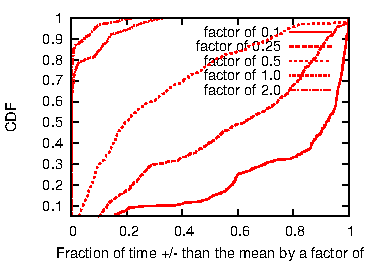
\includegraphics[width=0.4\textwidth] {figures/spatial-similarity.pdf}
\tightcaption{Spatial similarity of quality (average bitrate) among the sample of [Initial CDN, Initial Bitrate, ASN, Site, ConnectionType, Object].}
\label{fig:spatial-similarity}
\end{figure}

\myparasum{Spatial similarity} Spatial similarity is between the quality samples collected at the same time interval from sessions that share certain attribute values. \jc{Figure: x-Fraction of time less/greater than mean by various factor, y: CDF}

\begin{figure}[h!]
\centering
 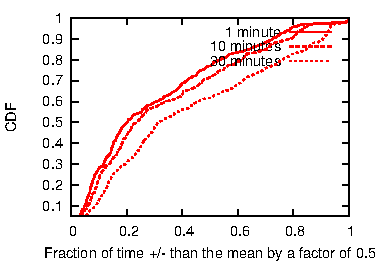
\includegraphics[width=0.4\textwidth] {figures/temporal-similarity.pdf}
\tightcaption{Quantifying impact of temporal noise on quality similarity. Figure shows likelihood of being more than a factor of 0.5 away from mean quality for all [Initial CDN, Initial Bitrate, ASN, Site, ConnectionType, Object] groups with increasing (from left to right) time scales.}
\label{fig:temporal-similarity}
\end{figure}

\myparasum{Temporal similarity} Temporal similarity is between the average quality collected in different time interval of the same group of sessions that share certain attribute values. \jc{Figure: x-Fraction of time less/greater than mean by various factor, y: CDF}

\myparasum{Summary of key observations} \jc{mostly based on my previous experience. subject to change after formal results are generated.}
\begin{packedenumerate}
	\item Both similarity of quality samples show that it is feasible to predict the quality of a new session and its decision by looking at quality samples that are spatially and temporally close to it.
	\item Spatial similarity varies across different attributes.  Using more attributes can improve things.
	\item Different quality metrics have different level of similarity, especially, buffering ratio has the largest similarity.
\end{packedenumerate}

\tightsubsection{Predicting from finite data}
Unfortunately, we do not have access to infinite data.  This is problematic because the mean quality outcome of a small sample of similar sessions (for example, $10$ such sessions) is subject to considerable random noise.  If we use that number for prediction, the prediction will be subject to the same noise and consequently to high average error.  As the number of attributes grows, quality grows more predictable (as we have seen) but the number of perfectly-matched sessions may drop exponentially.

Of course, prediction in the presence of limited information is the domain of statistics, and there are many potential solutions to this problem.  Any solution will deal with, and potentially trade off, four sources of prediction error:


\begin{figure}[h!]
\centering
\subfigure[Prediction error vs. group size (w.r.t average bitrate)]
{
        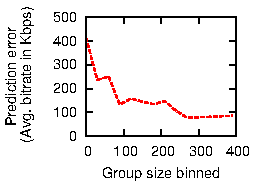
\includegraphics[width=110pt]{figures/count-err.pdf}
}
\subfigure[Distribution of group size]
{
        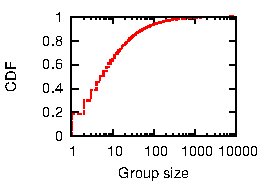
\includegraphics[width=110pt]{figures/count-cdf.pdf}
}
\tightcaption{Impact of group size (i.e., number of samples in a group). They show that more samples give more accuracy, and most of groups do not have sufficient samples for accurate prediction.}
\label{fig:group-size-impact}
\end{figure}

\begin{packedenumerate}
  \item \emph{Estimation error:} In the statistical literature, prediction error due to limited data is often called {\it estimation error}.  Other things being equal, more data produce more accurate prediction. For example, Figure~\ref{fig:group-size-impact}-(a) presents the prediction error of using a group as a function of its (i.e., number of samples). To show  In fact, estimation error is a serious practical problem for video quality prediction.  Using all available attributes, many sessions have very few matches, as we would expect given the exponential explosion in combinations of attribute values.  
  \item \emph{Bias} due to missing or unused information: When grouping sessions according to attributes we observe, we of course may not observe attributes that are important for prediction.  Say we do not observe (or use) important attribute X.  Then, even if we have infinitely many sessions that match the current session on all observed attributes, the average outcome for all of those sessions may be different from the average outcome for the subset of sessions that match the current session on attribute X.  This is a form of bias.  Predictability, as we have defined it, simply means low bias.  Importantly, it is not alleviated by gathering more session data; as we have seen, it may be alleviated by gathering more attributes about each session.
  \item \emph{Unavailability of recent data:} In a practical system, there are delays in sending and processing quality samples, so they are not available instantly.  If conditions change rapidly, there may be no quality samples sufficiently close to the session under prediction.  This is an extreme example of estimation error.  In this case it may be necessary to model the evolution of the video ecosystem over time in order to extrapolate to the current time.

\begin{figure}[h!]
\centering
 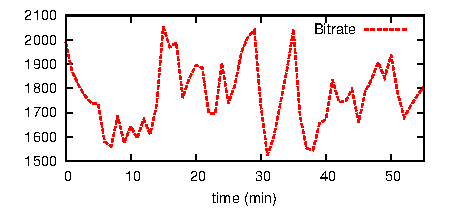
\includegraphics[width=0.4\textwidth] {figures/quality-time.pdf}
\tightcaption{Temporal variability of quality. The figure shows the mean value of average bitrate of a fixed group of same [Site, Initial CDN, Initial Bitrate, ConnectionType, ASN, Object], which has 100 quality samples in every minute in the figure.}
\label{fig:quality-variability}
\end{figure}

  \item \emph{Noise:} Even if we observed all conceivable attributes of a session and had infinitely many examples of exactly quality samples, outcomes may be affected by inputs that are practically random.  For example, performance may be affected by randomized algorithms in the networking layer.  This implies that some degree of prediction error is inevitable.
\end{packedenumerate}

More formally, we can derive this as follows (see \cite{domingos2000unified} for a less specialized discussion of the decomposition of prediction error).  Let $D$ be a set of quality samples from which a prediction algorithm learns its predictions.  Let $p_i$ be predicted quality for session $i$ and $q_i$ be its actual quality.  We further assume that $q_i$ is fixed except for an independent additive noise component, i.e. $q_i = \hat{q}_i + \epsilon_i$, where $\hat{q}_i$ is nonrandom and $\epsilon_i$ is a random variable with mean $0$, independent of $p_i$.  Then the expected squared prediction error, with respect to randomness in the observed data $D$ used to compute $p_i$, is:
\begin{align*}
  \E_D[(p_i - q_i)^2] &= \Var_D[p_i - q_i] + (\E_D[p_i - q_i])^2 \\
  &= \Var_D[p_i - \hat{q}_i - \epsilon_i] + (\E_D[p_i - \hat{q}_i - \epsilon_i])^2 \\
  &= \Var_D[p_i - \hat{q}_i] + \Var_D[\epsilon_i] + (\E_D[p_i - \hat{q}_i - \epsilon_i])^2\\
  &= \Var_D[p_i] + \Var_D[\epsilon_i] + (\E_D[p_i - \hat{q}_i - \epsilon_i])^2\\
  &= \Var_D[p_i] + \Var_D[\epsilon_i] + (\E_D[p_i - \hat{q}_i] - \E_D[\epsilon_i])^2\\
  &= \Var_D[p_i] + \Var_D[\epsilon_i] + (\E_D[p_i] - \hat{q})^2
\end{align*}

The first term is estimation error -- the variability in predictions across possible sets of observed data.  It will increase as the number of sessions similar to session $i$ in $D$ decreases; as a special case it may be very large if only a few quality samples in $D$ are temporally close to session $i$.  The second term is noise.  The third term is the squared bias of the predictor, which does not generally decrease with the size of $D$.  The prediction algorithm's average prediction error is simply the average over all sessions $i$ of the sum of these three terms.

\tightsubsection{Aggregation}
A simple strategy to reduce estimation error is {\it aggregation}.  By aggregation we mean putting sessions into coarser groups that match on only a subset of observed attributes.  Aggregation increases the number of samples in each group but reduces the number of attributes, thus reducing estimation error at the cost of increased bias.  Thus it makes sense to look for an optimal degree of aggregation.  Figures \fillme show that the optimal AC (the aggregation that gives minimal prediction error) is in many cases neither the finest nor the coarsest one.



\begin{figure}[h!]
\centering
 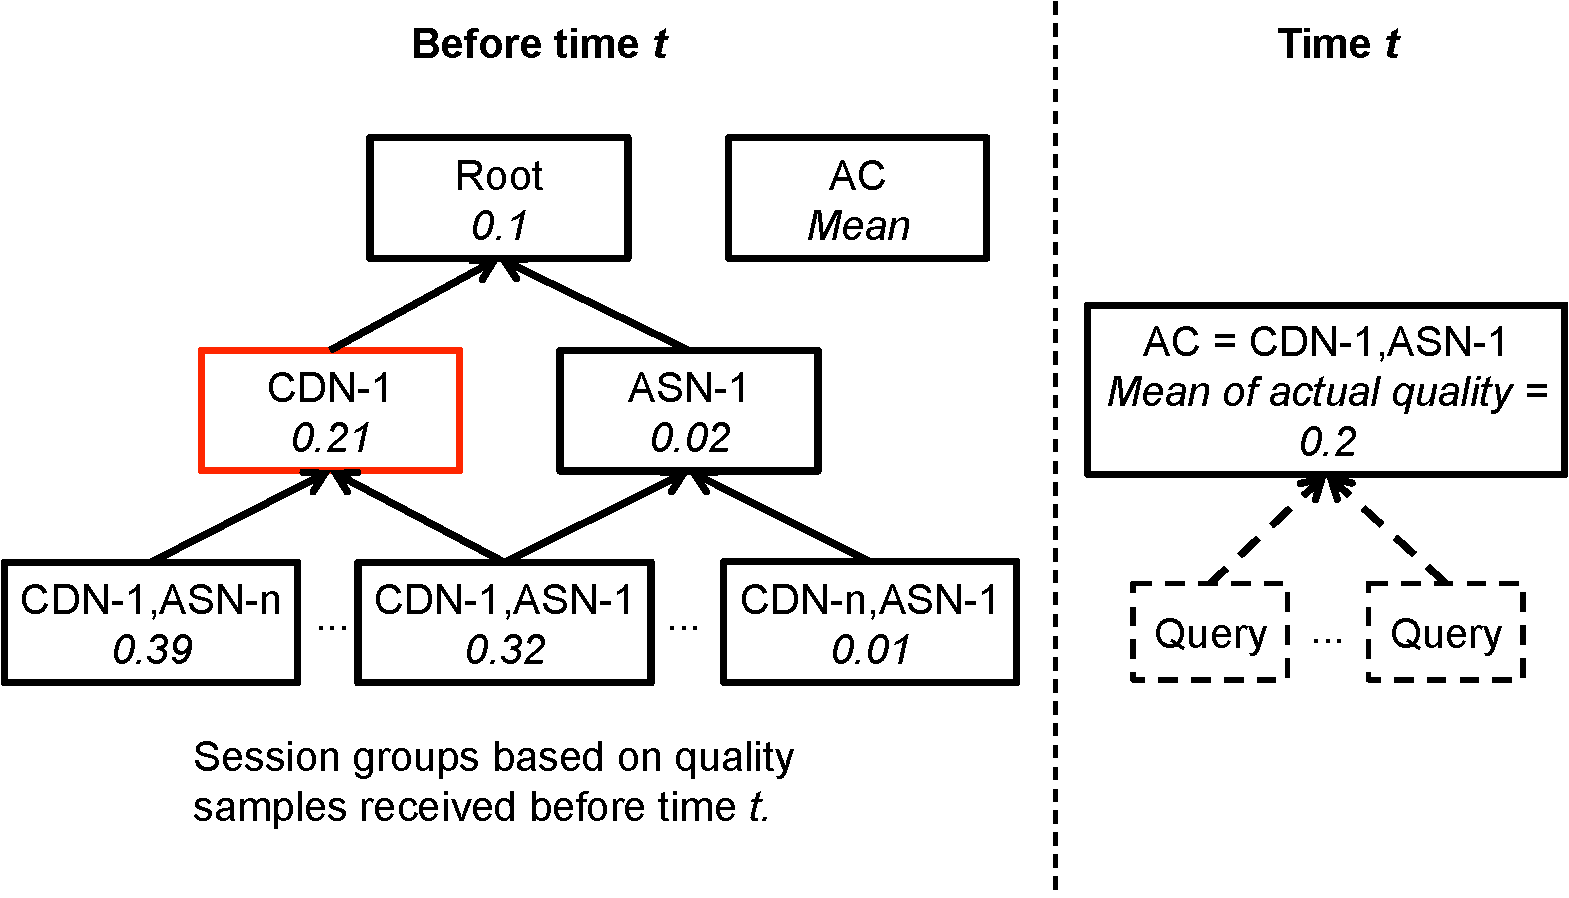
\includegraphics[width=0.5\textwidth] {figures/fig-optimal-AC.pdf}
\tightcaption{Example of how optimal AC is identified. The optimal AC is colored in red. Assuming the considered attributes are fixed, the optimal AC assumes that all sessions that belong to the same finest group should be given the same prediction, and the optimal AC is the one that gives the closest prediction among those that contain this finest group.}
\label{fig:example-optimal-ac}
\end{figure}

Figure~\fillme-(a) shows for each AC, the fraction of sessions for which it is the optimal AC with respect to average bitrate. We use ``CDN, starting bitrate, connection type, ASN'' as attributes and always look at one-minute history, in order to avoid impact of temporal aggregation. The figure shows that there is no dominant AC that is optimal for most of the sessions; Even the top five most frequent optimal ACs only count for less than \fillme of sessions. Figure~\fillme-(b) shows the frequency of the top five most frequent optimal AC over the period of \fillme hours. The figure shows that their frequency also changes with substential variability, which suggests that optimal AC must be chosen adaptively.
Therefore, there is no universal optimal AC or a set of ACs that can produce best prediction for even most of sessions. Moreover, in most cases, the optimal AC is neither the finest nor the coarsest AC.



\begin{figure}[h!]
\centering
\subfigure[Distribution of optimal AC. No single or small set of ACs can be used as optimal AC for most quries.]
{
        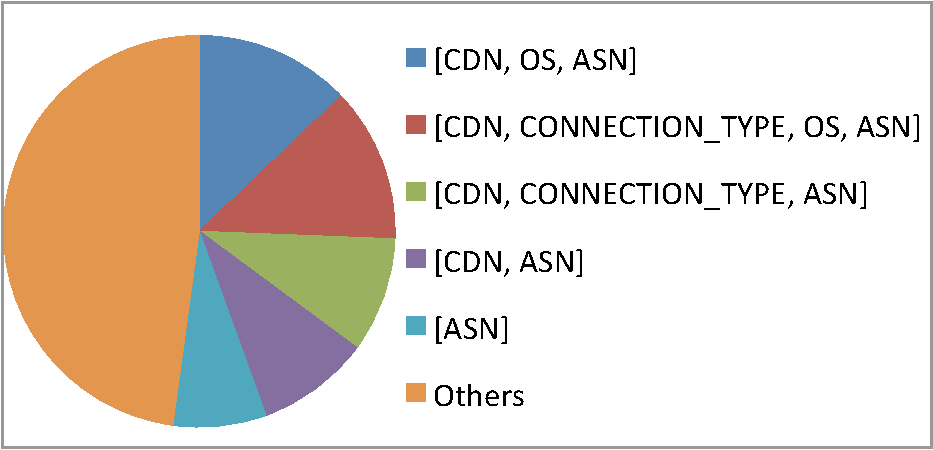
\includegraphics[width=0.4\textwidth]{figures/optimal_AC_distribution.pdf}
}
\subfigure[Prevalence of pair of (finest group, optimal AC). 70\% pairs of (finest group, optimal AC) only last for less than 20\% of time.]
{
        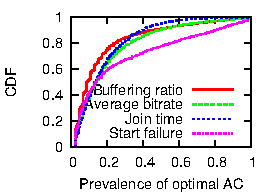
\includegraphics[width=0.4\textwidth]{figures/optimal-prevalence.pdf}
}
\tightcaption{Dynamics of the optimal AC. Prevalence of pair of (finest group, optimal AC) is the fraction of time that the finest group has this optimal AC.}
\label{fig:optimal-ac-dynamics}
\end{figure}

When estimation error is small (say, when a fine-grained group contains many sessions) we want to eliminate bias by using a fine-grained group.  When estimation error is large, we want to aggregate more.  Figure \fillme demonstrates this for \fillme.  This indicates that a prediction algorithm that uses aggregation should pay attention to its error rate to determine the right degree of aggregation.

\tightsection{Prediction algorithms}
\label{prediction}
The tradeoff between estimation error and bias via aggregation naturally leads us to consider a class of algorithms that compute average quality outcomes for groups of sessions under different attribute sets, and then {\it dynamically} choose the attribute set that seems to work well for a particular session under prediction.  Since it is difficult to find the best attribute set, it is useful to hedge our bets by taking a weighted combination of averages.  George et al \cite{george2008value} consider this problem and propose the following algorithm for choosing the weights.  For a session under prediction having index $i$, let $a_i$ be the tuple of all attributes observed for that session and let $q_i$ be its quality outcome.  For each attribute set $g$ in our collection of attribute sets $G$, define a function $v_g$ that picks out those attributes:
\begin{equation*}
  v_g(\cdot): a \mapsto \text{[the subtuple of $a$ containing attribute values for the attributes in g]} .
\end{equation*}
We first compute the single-group average quality outcome for each $g$:
\begin{align*}
  \bar{q}_{g}(a_i) &= \frac{1}{N_{g}(a_i)} \sum_{j \in N_{g}(a_i)} q_j, \text{ where} \\
  N_{g}(a_i) &= |\{j: v_g(a_j) = v_g(a_i), j < N\}|
\end{align*}
Then, considering $\bar{q}_{g}(a_i)$ as an estimate of $q_i$, estimate its mean squared prediction error $e_{g}(a_i)$.  This estimation step is not simple, so we will briefly postpone its description.  Having computed $\bar{q}_{g}(a_i)$ and $e_{g}(a_i)$ for each attribute set, our final quality prediction, which we denote $\bar{q}(a_i)$, is the weighted average of $\bar{q}_{g}(a_i)$, where the weights are equal to the inverse of $e_{g}(a_i)$, normalized to sum to $1$:
\begin{align*}
  \bar{q}(a_i) = (\sum_{g \in G} e_{g}(a_i)^{-1})^{-1} \sum_{g \in G} e_{g}(a_i)^{-1} \bar{q}_{g}(a_i) .
\end{align*}

$e_{g}(a_i)$ is estimated by separately estimating (squared) bias and estimation error and summing them, plugging them into equation \eqref{eqn:biasvariance}.  Bias is heuristically taken to be the difference between the finest-granularity estimate of $q_i$ (i.e. $\bar{q}_{g'}(a_i)$, where $g'$ is the finest-grained ACS) and $\bar{q}_{g}(a_i)$.  Variance is estimated by a standard formula:
\begin{align*}
  \frac{1}{N_{g}(a_i)} \sum_{j \in N_{g}(a_i)} (q_j - \bar{q}_{g}(a_i))^2
\end{align*}

George et al call the resulting prediction algorithm WIMSE, for Weighted Inverse Mean Squared Error.  Inverse-mean-squared-error weighting has the following nice property: If each $\bar{q}_{g}(a_i)$ is statistically independent, then $\bar{q}$ is an optimal estimator in the sense that it has minimal mean squared error among all functions of \cite{}.  However, in our setting (and in the original motivating setting) the $\bar{q}_{g}(a_i)$ are based on overlapping data and are therefore not independent.  Further, our estimates of both the bias and variance components of $e_{g}(a_i)$ are imprecise.  Thus we have no neat theoretical guarantee of optimality for WIMSE, though George et al find that WIMSE can nevertheless work well.  The deficiencies of the algorithm necessitate a few tweaks in our setting, which we now present.

\begin{figure*}[t!]
\centering
\subfigure[Exhaustive vs. greedy (GO) search]
{
        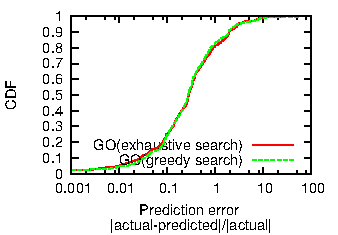
\includegraphics[width=0.3\textwidth]{figures/prediction-comparisons/example-exhaustive-metric1.pdf}
}
\subfigure[GO vs. variants]
{
        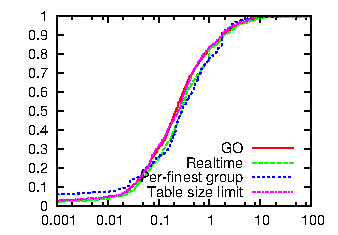
\includegraphics[width=0.3\textwidth]{figures/prediction-comparisons/example-acs-metric1.pdf}
}
\subfigure[GO vs. oracle (optimal AC)]
{
        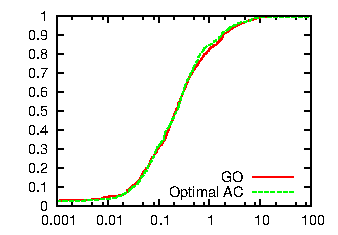
\includegraphics[width=0.3\textwidth]{figures/prediction-comparisons/example-oracle-metric1.pdf}
}
\tightcaption{Comparison between GO ACS selection with other strawmans (considerd quality metric is average bitrate).}
\label{fig:acs-comparison}
\end{figure*}

\tightsubsection{ACS selection}
One difficulty faced by a user of WIMSE is selection of the ACS.  WIMSE may not perform best when given the power set of possible ACs because the independence assumption is dramatically violated.  For example, if two ACs produce similar groups, then both will receive similar weights; including both ACs doubles the weight of the corresponding groups for no principled reason.  Another reason to choose ACs carefully is that many of the computational costs of WIMSE scale with the number of groups; we discuss this further in \Section~\ref{sec:scalability}.

\myparasum{Greedy static ACS selection and strawmans} We take a data-driven approach to ACS selection. We separate part of historical sessions as test set and best ACS selection is the one that gives the best average accuracy over the test set using WIMSE. 

\myparasum{Justify greedy algorithm} One problem with this approach is that even in offline analysis, the potential space to search for the best ACS is too huge (with $k$ attributes, there will be $2^k$ ACs, and in total $2^{2^k}$ ACSes). Instead, we first examine a greedy algorithm which find a good ACS in $O(2^k)$ amount of steps, and compare it against exhaustive search result with $k=3$ attributes (i.e., 256 ACSes). Figure~\ref{fig:acs-comparison}-(a) presents the CDF of prediction accuracy w.r.t average bitrate of the ACS that obtained by exhaustive search and greedy search. It shows that the ACS they choose, though different, can offer similar quality of prediction.

\jc{Pseudo code of greedy ACS selection.}

\myparasum{Per-finest group selection vs. one global ACS} One strawman for our algorithm to compare with is one where the selected ACS can be different for different sessions. Especially, if two sessions differ in at least one attribute, they can use different ACS. \fillme. \jc{Results shown in Figure~\ref{fig:acs-comparison}-(b), and they perform similarly and the global ACS performs even slightly better, possibly because per-finest-group ACS has side-effect of overfitting.}

\myparasum{Oracle approach vs. historical based} \fillme. \jc{Results shown in Figure~\ref{fig:acs-comparison}-(b). Result needs to be changed after discussion today.}

\tightsubsection{Pseudocount priors}
That algorithm assumes that bias and variance can be computed exactly, while in practice variance cannot be estimated accurately when groups are very small.  To alleviate this, we use a simple idea from Bayesian statistics: We incorporate a prior distribution on quality outcomes within each group.  This amounts to adding a few fake ``pseudocount'' observations to each group.  \fillme.


\begin{figure}[h!]
\centering
 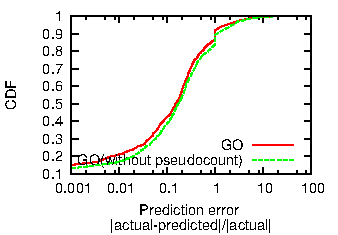
\includegraphics[width=0.4\textwidth] {figures/prediction-comparisons/example-pcount-metric1.pdf}
\tightcaption{GO with pseudocount vs. without pseudocount (considerd quality metric is average bitrate).}
\label{fig:quality-variability}
\end{figure}

For each of these we should have a CDF of errors and also the average prediction error.
\begin{itemize}
	\item GO with greedy ACS selection and pseudocount priors
	\item GO with greedy ACS selection and no pseudocounts
\end{itemize}

\tightsubsection{Mini-evaluation of prediction accuracy}
Given an ACS selection algorithm, we’re going to use all attributes we have and test GO prediction accuracy against two simple baselines.
\begin{itemize}
	\item GO with greedy ACS selection and pseudocount priors
	\item Predict using average of last 2 hours on all traffic for this CDN
	\item Predict using average of last 2 hours on the finest group that has any data
\end{itemize}
For each of these we should have a CDF and also display the average prediction error.

\begin{figure*}[t!]
\centering
\subfigure[Buffering ratio]
{
        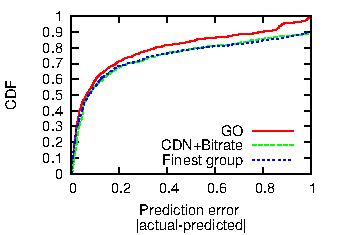
\includegraphics[width=0.22\textwidth]{figures/prediction-comparisons/example-naive-metric0.pdf}
}
\subfigure[Average bitrate]
{
        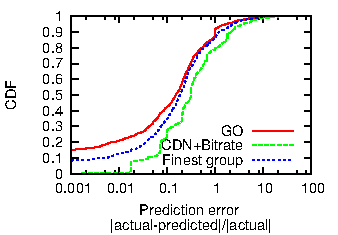
\includegraphics[width=0.22\textwidth]{figures/prediction-comparisons/example-naive-metric1.pdf}
}
\subfigure[Join time]
{
        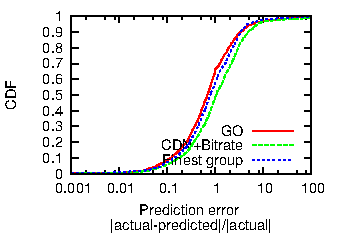
\includegraphics[width=0.22\textwidth]{figures/prediction-comparisons/example-naive-metric2.pdf}
}
\subfigure[Start failure]
{
        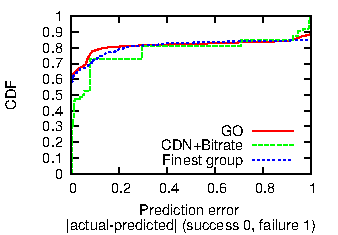
\includegraphics[width=0.22\textwidth]{figures/prediction-comparisons/example-naive-metric3.pdf}
}
\tightcaption{Comparison between GO and two baseline approaches where the selection and use of ACS is statically used -- (1) no attributes considered except (CDN, bitrate), (2) all attributes considered.}
\label{fig:compare-to-naive}
\end{figure*}

\henry{The following two subsections contain a bunch of caveats.  It might be more effective to move them to a later section on future work.}

\tightsubsection{Interactions between decisions}
The reader may be bothered by a simplifying assumption implicit in our characterization of the causes of prediction error.  If we allocated all traffic to a single CDN, its performance might degrade, but our session-wise prediction does not capture that.  We might instead want to know the following: Given a set of decisions about sessions (say, all the sessions we observe in a 1-hour interval), what is the predicted performance for that set of sessions?  We do not wish to say that such a question is impossible to answer, but rather point out some difficulties in answering it, and some reasons why it is less critical to answer it than it may appear.

Joint prediction is statistically difficult because existing statistical prediction algorithms typically assume the performance of training examples are independent and experience identical randomness (i.e. they are IID).  We observe very few IID instances of whole sets of sessions; in our example, we observe only one per 1-hour interval.  It is possible to model explicitly the dependence of each session’s performance on the set of joint decisions, but this requires modeling choices that we may not make well, and such models are typically computationally expensive to learn. \fillme

If conditions change slowly enough, the independence assumption is not so bad.
The rate of change of CDN allocations is naturally limited for our problem by the rate of session arrivals, since we choose CDNs only at the beginning of each session.  Spikes in the rate of new sessions are not typically high enough to necessitate special handling.  \henry{Need some data and experiments for this.  Davis or Florin have done some of the experiments, I think.}

\tightsubsection{Alternative approaches}
The reader should not leave with the impression that the algorithm described above is the only possible one for predicting video quality, or even the best.  The scope of this paper is merely to establish a reasonable approach and show that it results in improvements.  Other possible approaches might include:
\begin{packedenumerate}
  \item \emph{Linear regression:} After encoding categorical attributes as binary features, simple linear regression can be applied to predict quality outcomes.  Temporal attributes can be passed through nonlinear functions to achieve reasonable time-series prediction.  Interaction terms (e.g. the indicator for a session coming from ASN $100$ multiplied by the indicator for the session having Object ``foo'') can simulate attribute combinations, at the cost of a combinatorial explosion in the size of the learned model.  However, recent developments in optimization for $\ell_1$-regularized linear regression allow models to be learned quickly online while providing the guarantee that the learned model is \emph{sparse}, i.e. that only a few important features are selected for inclusion in the model and the rest can be safely dropped.  See \cite{duchi2010composite} for one example of work that could enable this technique.  One downside is that linear models are harder to interpret than a model based on averaging group averages.
  \item \emph{Hierarchical Bayesian modeling:} In this approach, groups are placed in the natural tree, and each is associated with a probability distribution over quality outcomes, such as a Gaussian distribution.  Each group inherits information from the distribution of its parent group in the form of a prior.  Such models potentially deal very naturally with data sparsity and with dependence among sessions \cite{gelman2003bayesian}, but learning them from data is often computationally intractable.
\end{packedenumerate}

\tightsection{Quality Improvement via Prediction}
\label{improvement}
%Now we can fill in the details of section 3 a bit more.  Figure~\ref{fig:go-overview} shows how prediction and decision-making work in GO.
Having shown that with the attributes we collect, our prediction algorithms can provide close-to-optimal prediction accuracy, we now examine the quality improvement resulting from the prediction algorithms. Providing that our prediction algorithm is roughly accurate, GO's ``transition'' from prediction accuracy to quality improvement is straightforward -- it simply chooses the decision that has the best predicted quality. 

Since improving video quality is the ultimate goal of GO, we would like to quantify the impact of prediction algorithms on quality improvement. Specifically, we would like to answer two questions:
\begin{packedenumerate}
	\item How much quality improvement does GO make under various scenarios?
	\item How does prediction accuracy impact quality improvement under realistic scenarios?
\end{packedenumerate}

The difference between two questions is that the first question quantifies the impact of different scenarios on quality improvement with a fixed solution, i.e., GO. The second question quantifies the impact of the goodness of solution (i.e., prediction accuracy) on quality improvement, in realistic scenarios. This section begins with our methodology to answer the two questions. Then, we present our results and observations of each question.

\tightsubsection{Methodology}
To answer these two questions, we need to have three types of input. Here we briefly describe their intuition and difference. We will present the parameters and setup in detail when using them to answer particular questions.
\begin{packeditemize}
	\item {\it Controlled synthetic input:} We need fully controlleable input in which the true outcomes (i.e., ``ground truth'') of multiple decisions are under our control and we can change them continously so as to quantify the quality improvement. By doing so, we would also be able to have access to the optimal quality (i.e., an {\it oracle} approach) which it will be useful to compare GO with.
	\item {\it Counterfactual input:} To answer these questions under realistic scenarios (real trace), we use a methodology similar to A/B testing, which we call {\it counterfactual testing}. The methodology is described in detail in section~\ref{sec:counterfactualtesting}. Its basic idea is that we first collect a dataset (called {\it random dataset}) in which the decisions are randomly made for each client and we collect the quality each client gets. To evaluate the outcome of the same set of sessions with each making a decision based on some algorithm (i.e., possibly the same decision), we will be able to have unbiased evaluation on those sessions with the same decision as in the dataset.
	\item {\it Randomized trace-driven input:} Randomizing real traces with controlled amount is important for evaluating a decision-making algorithm. However, real traces do not admit the sensitivity analysis of a decision-making algorithm to the changes in scenario parameters -- after the input scenarios is changed, the outcome of each session under an alternative decision is unavailable \jc{why counterfactual input won't work}.  To remedy these limitations, we generate a trace-driven synthetic dataset. The basic idea is to generate a session $s$ whose outcome of each decision $d$ is drawn from the distribution of outcomes of this decision $d$ on other sessions exactly matching the same attributes with $s$. Having ensured that quality outcomes in the synthetic scenario are known for any decision, it is possible to identify an {\it oracle} approach that always makes the best decision.
\end{packeditemize}
In any scenario, we would like to quantify the quality improvement of GO based on random selection (which makes decision with equal prabability), and how close GO is to an oracle approach (with controlled and trace-driven synthetic input).

\comment{
\begin{figure}[h!]
\centering
 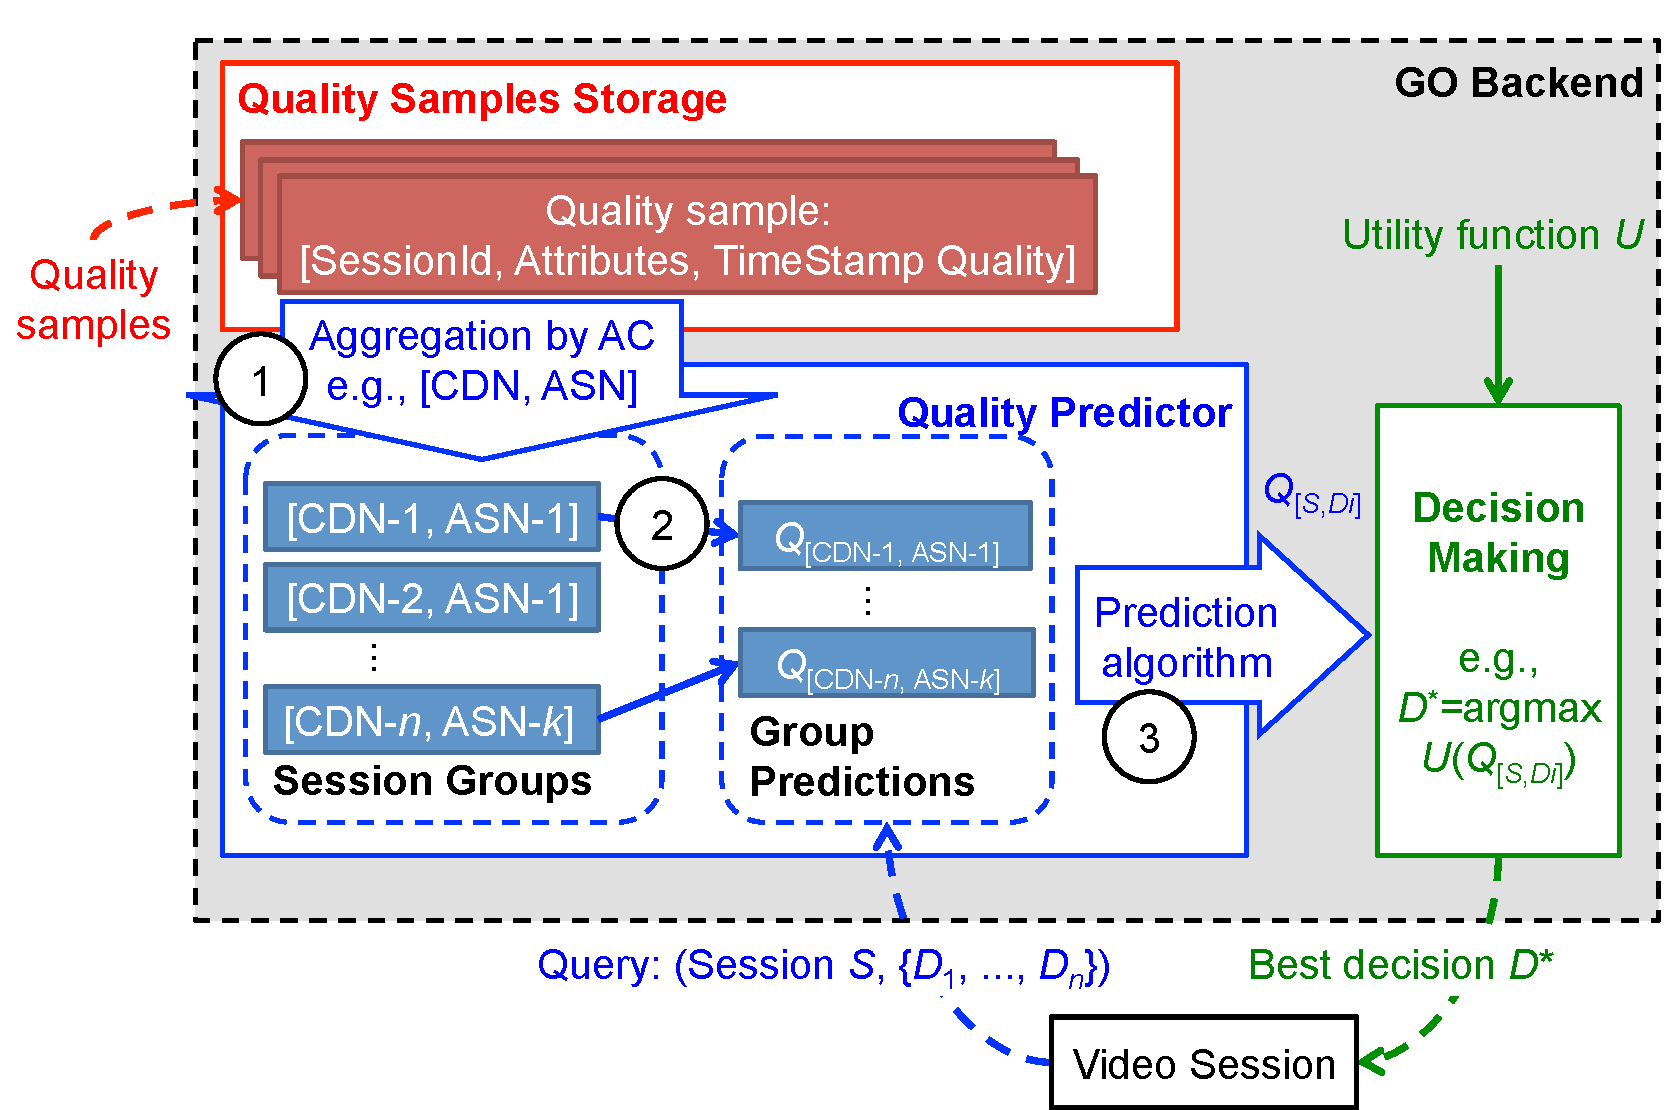
\includegraphics[width=0.3\textwidth] {figures/backend.pdf}
\tightcaption{Schematic overview of GO backend.}
\label{fig:backend}
\end{figure}
}

\tightsubsection{Improving quality with GO}

\tightsubsubsection{Behavioral study}
To build confidence in this algorithm, we use controlled synthetic input to show how decision-making based on prediction behaves in some simple synthetic scenarios where the optimal decisions are clear:
\begin{packedenumerate}
  \item {\it CDN performance degradation.} A sudden change in performance of one group causes GO to switch decision accordingly. Figure~\ref{subfig:behavioral:cdn} shows the behavior of sessions in one ASN when provided with two CDNs to choose from. Assume that buffering ratio is the only considered quality metric. The average buffering ratio of CDN1 is stably at 0.2 and that of CDN2 changes between 0.1 and 0.25.
  \item {\it Dynamic bottleneck.} Performance of group A is decided by client-side problem, and that group B is decided by CDN-side problem, so when CDN changes its performance, only group B will switch decision.
\end{packedenumerate}

\begin{figure*}[t!]
\centering
\subfigure[CDN performance degradation]
{
        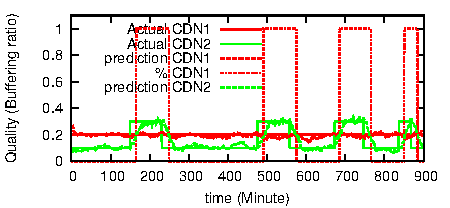
\includegraphics[width=0.4\textwidth]{figures/behavior-evaluation/simple-change.pdf}
	\label{subfig:behavioral:cdn}
}
\subfigure[Impact of bottlenecks]
{
        
\includegraphics[width=0.4\textwidth]{figures/placeholder.pdf}
	\label{subfig:behavioral:bottleneck}
}
\tightcaption{Behavioral study.}
\label{fig:behavioral}
\end{figure*}


\tightsubsubsection{Evaluation under real trace}
We show how GO works in practice in a real trace, in comparison to a naive baseline algorithm that makes random decisions.  Here we use a methodology similar to A/B testing, which we call {\it counterfactual testing}; the methodology is described in detail in section \ref{sec:counterfactualtesting}.  The dataset is described in section \ref{subsec:dataset}.  Results are displayed in figure \fillme; we can see that \fillme.

\begin{figure*}[t!]
\centering
\subfigure[Buffering ratio]
{
        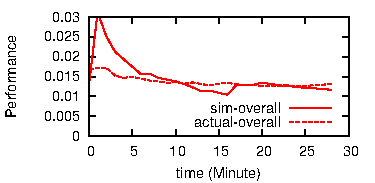
\includegraphics[width=0.23\textwidth]{figures/counterfactual/result-a-overall-metric0.pdf}
}
\subfigure[Average bitrate]
{
        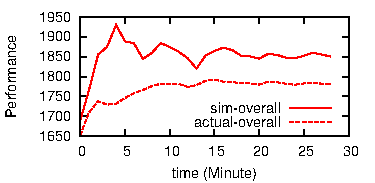
\includegraphics[width=0.23\textwidth]{figures/counterfactual/result-a-overall-metric1.pdf}
}
\subfigure[Join time]
{
        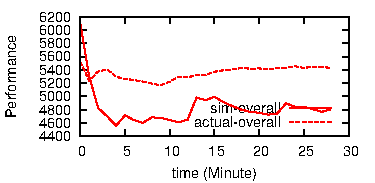
\includegraphics[width=0.23\textwidth]{figures/counterfactual/result-a-overall-metric2.pdf}
}
\subfigure[Start failure rate]
{
        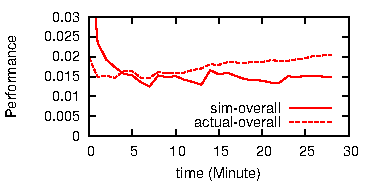
\includegraphics[width=0.23\textwidth]{figures/counterfactual/result-a-overall-metric3.pdf}
}
\tightcaption{Counterfactual input. Evaluation under real trace}
\label{fig:counterfactual}
\end{figure*}

\tightsubsubsection{Impact of quality heterogeneity}
To control the quality heterogeneity, we randomize the real trace to create a randomized trace-driven input. \fillme \jc{it's still not clear to me how we change the quality outcome}



%Randomized experimentation in real traces is the most important way to evaluate a decision-making algorithm.  However, real traces have a few limitations.  In real traces, it is impractical to identify an optimal alternative against which to compare GO, so that we can understand how close it is to the best algorithm.  In addition, real traces do not admit simple analysis of the sensitivity of a decision-making algorithm to the changes in scenario parameters.  To remedy these limitations, we generate a synthetic dataset from our real data.  We do this using a simplifying assumption: We fix a set of attributes $g$, and assume that conditional on a session belonging to a group under this AC, its quality outcomes given each decision are statistically independent.  Essentially this amounts to an assumption that we observe all interesting attributes.  \fillme.

%Under this assumption, we can generate a new session from the same distribution that generated a real dataset as follows: Sample uniformly at random from the sessions we observed.  The synthetic session has the same attributes, denoted $a_i$, as the sampled session.  We assign quality outcomes to each possible decision by sampling uniformly at random from the quality outcomes observed for sessions with attributes exactly matching $a_i$.  Crucially, this ensures that quality outcomes in the synthetic scenario are known for any decision, not just the decision that was actually taken for a session.  In particular, it is possible to identify an {\it oracle} for this scenario that makes perfect predictions of quality outcomes for any decision.

% [The following is an unfinished writeup for old synthetic scenario scheme:]
%The scenario is generated as follows: The scenario lasts for $T$ minutes.  Each session is assigned values on four different attributes, $A_0, A_1, B_0,$ and $B_1$, and lasts for $1$ minute.  Each unique attribute combination (i.e. each group) $a$ is associated with some static parameters and some parameters that change over time, which inform the generation of sessions in that group:
%\begin{packedenumerate}
%  \item $n_{a}$: The number of sessions in this group.
%  \item $\mu_{atj}$: The average quality outcome for sessions in this group, when decision $j$ is taken.
%  \item $\sigma_{atj}$: The standard deviation of quality outcomes for sessions in this group, when decision $j$ is taken.
%\end{packedenumerate}
%
%For each minute $t$, sessions are generated as follows: Group $a$ has $n_{a}$ sessions.  The $i$th session in group $a$ has attribute values $a$.  There are $J$ possible decisions; each session has quality outcome $q_{itaj}$ drawn from the distribution $\operatorname{Normal}(\mu_{atj}, \sigma_{atj}^2)$, for each decision $j$.  The actual decision $d_{ita}$ for the session, which is used to populate the quality sample used in GO, is chosen uniformly at random from among the $J$ possible decisions.

%\tightsubsubsection{Evaluation against an oracle using synthetic data}
%Here we compare GO against the oracle (and against a random decision-maker) in our synthetic scenario.  \fillme.
%
%We also check the sensitivity of GO to the true difference in quality between decisions.  We do this by shifting the distribution of true quality outcomes in varying degrees.  \fillme.

\tightsubsection{Understanding the impact of prediction accuracy on quality improvement}

Separately from the GO algorithm, it is also interesting to see how prediction error generically impacts quality outcomes.  To control the prediction accuracy in real trace, we have to identify the true outcome of decisions we did not take. Therefore, we use randomized trace-driven input. The key challenge is given a session $s$ and one of its decisions $d$, to draw the outcome from the distribution $M_{v_g(s),d}$ of outcomes of this decision on other sessions that share the same attributes with this session. Remember $v_g(s)$ returns the values on all attributes in $g$ of session $s$. We investigate two ways of doing so. 
\begin{packedenumerate}
	\item Unproprtional: The outcome is uniformly at random from $M_{v_g(s),d}$. Its underlying assumption is that we observe all attributes that determine the quality, so that with the same decision, the quality of sessions that match all attribute is random values with unbias noise.
	\item Proportional: For a session $s$, if the outcome of $d_1$ is in the $q$-quantile of $M_{v_g(s),d_1}$, the outcome of $d_2$ is also in the $q$-quantile of $M_{v_g(s),d_2}$. Its underlying assumption is that there is unobserved attributes that determine the quality, so that if the session performs poorly in one decision, it will also be bad on other decisions.
\end{packedenumerate}

We control the prediction accuracy by generating prediction such that the prediction deviates from the real outcome by an independent random Gaussian noise of varying magnitude. (multiplicative)

\begin{figure}[h!]
\centering
 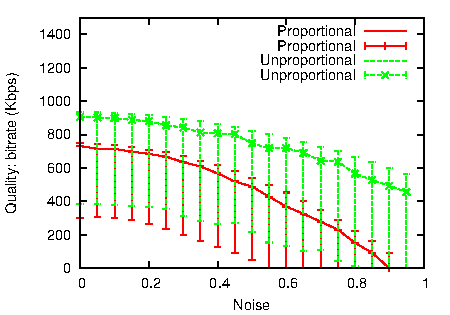
\includegraphics[width=0.3\textwidth] {figures/impact/result-noise-impact.pdf}
\tightcaption{Impact of noise on quality improvement (Y axis) based on random selection. GO prediction gives 830Kbps (unproportional) and 780Kbps (proportional), roughly identical to noise of gaussian random noise of standard deviation of 0.5.}
\label{fig:cdn-degradation}
\end{figure}

%Here it is important to identify an oracle predictor as a baseline, so we use the same synthetic scenario as above.  We add random independent Gaussian noise to the oracle's predictions (an admittedly crude model of prediction error) and show how larger amounts of noise impact quality outcomes.  Figure \fillme displays this.  We can see that quality improvement is unaffected by small amounts of prediction inaccuracy but drops off quickly at a (scenario-dependent) threshold \fillme.

%We cannot subtract noise from GO's predictions in a real scenario, since we do not know the true outcome of decisions we did not take.  However, we can {\it add} noise to GO's predictions and observe the impact of {\it worse} prediction on quality outcomes.  As above, we use independent random Gaussian noise of varying magnitude.  Figure \fillme displays this for our synthetic scenario, and figure \fillme displays it for a real trace.  In the synthetic scenario, GO's performance in quality improvement is equivalent to that of an oracle with \fillme random noise.  \henry{We hope to see that decreasing prediction accuracy eventually leads to highly degraded performance.}

\tightsection{Implementation and Scalability}

In this section, we present the high level GO implementation. While there are much details in GO system, we focus on the two main components: data processing and decision making. Paramount in our implementation was the need to make very rapid decisions, as any extra delay in decision making could impact performance of the client making the request. This meant that the vast majority of prediction information needed to be precomputed. This resulted in an implementation that involves two parts: computation of a group table, and broadcasting of said table out to servers close to the clients making requests.

%The GO backend collects information (including quality samples) sent back by clients, processes the information periodically to aggregate the information, and then, upon on receiving a request from a new session, the best decision can be made quickly.

%Like many data processing systems, individual events from every single client sending information must be rolled up and summarized into a succinct format. Because many systems do this, and there is nothing specific to our problem about how this is done, we will focus on how the system rapidly translates these summaries into meaningful pieces of information used for prediction and decision making. These summaries consist of the most recent performance information about a session, as well as the information about what decision was made for the session. 

\myparatight{Creating group table} Group table generation is essentially the process of aggregating samples into buckets, and then computing summary statistics for each bucket.  Our implementation uses Spark as the underlying compute framework, and the problem can be captured in a single map-reduce stage. Data samples are loaded in parallel from an HDFS source and distributed amongst the cluster. Each node then maps its share of samples to a set of preliminary buckets. Common buckets are then shuffled across the cluster and the results are aggregated and collected onto a master machine. See Figure~\ref{fig:computing-scale}

\begin{figure}[h!]
\centering
 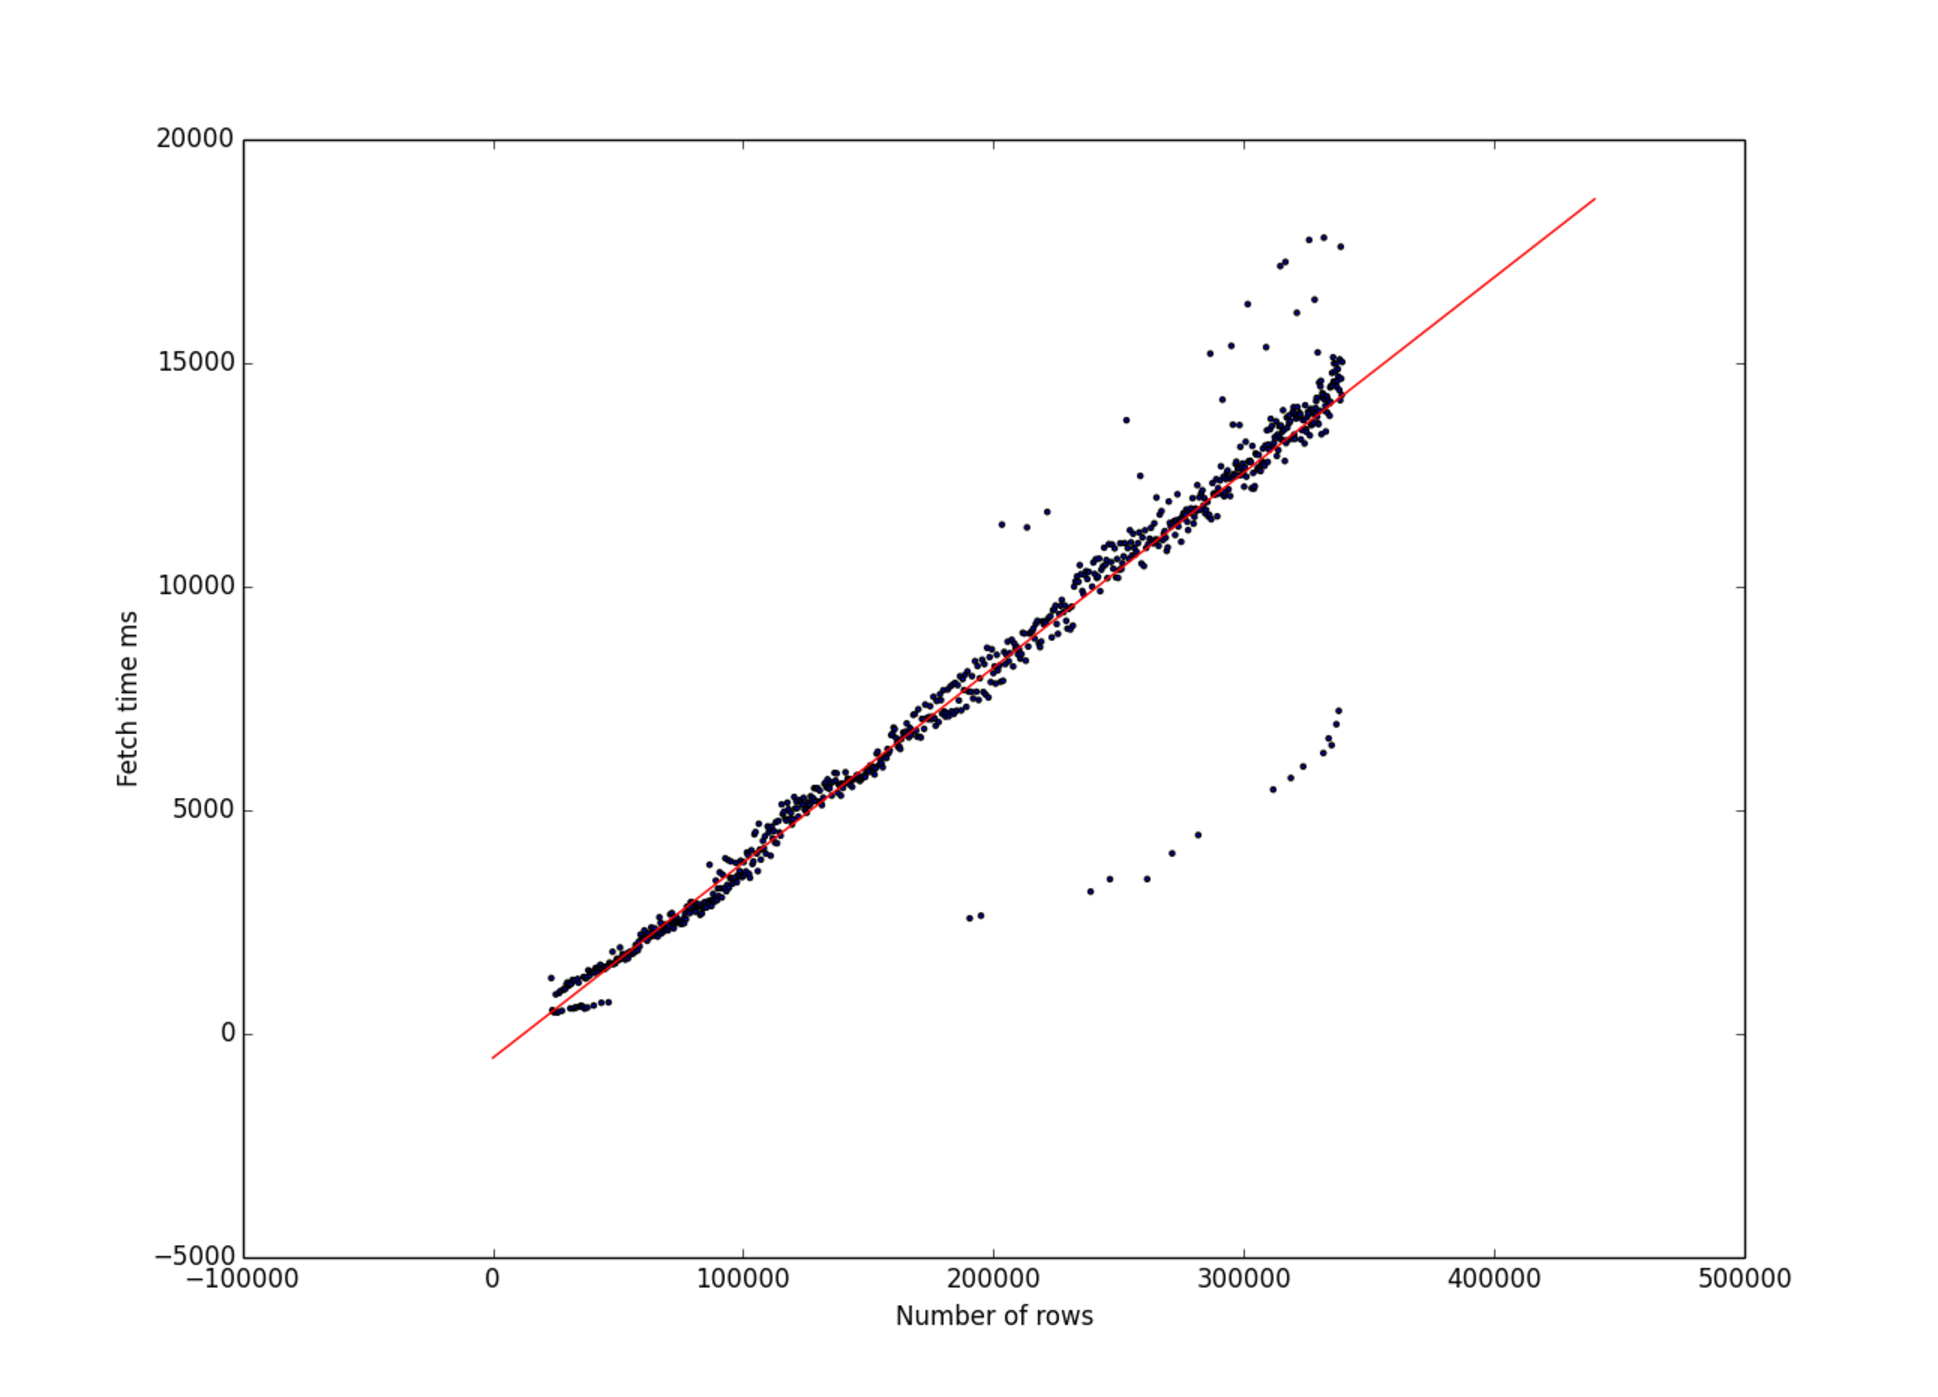
\includegraphics[width=0.5\textwidth] {figures/scale/fetch_time_scale.pdf}
\tightcaption{Dummy figure. This will essentially be overlaid multiple scatter plots from different cluster
sizes to show that increasing cluster size improves computation time}
\label{fig:computing-scale}
\end{figure}

\myparatight{Broadcasting group table} The resulting table is broadcasted wholesale out to a larger group of decision makers (DMs) closer to video clients in multiple POPs by way of a distributed messaging system, Kafka. The bottleneck here is bandwidth, as the table can be quite large.  In general is is an $O(n)$ process to deliver the table where $n$ is the number of distinct rows. See Figure~\ref{fig:fetching-scale}

\begin{figure}[h!]
\centering
 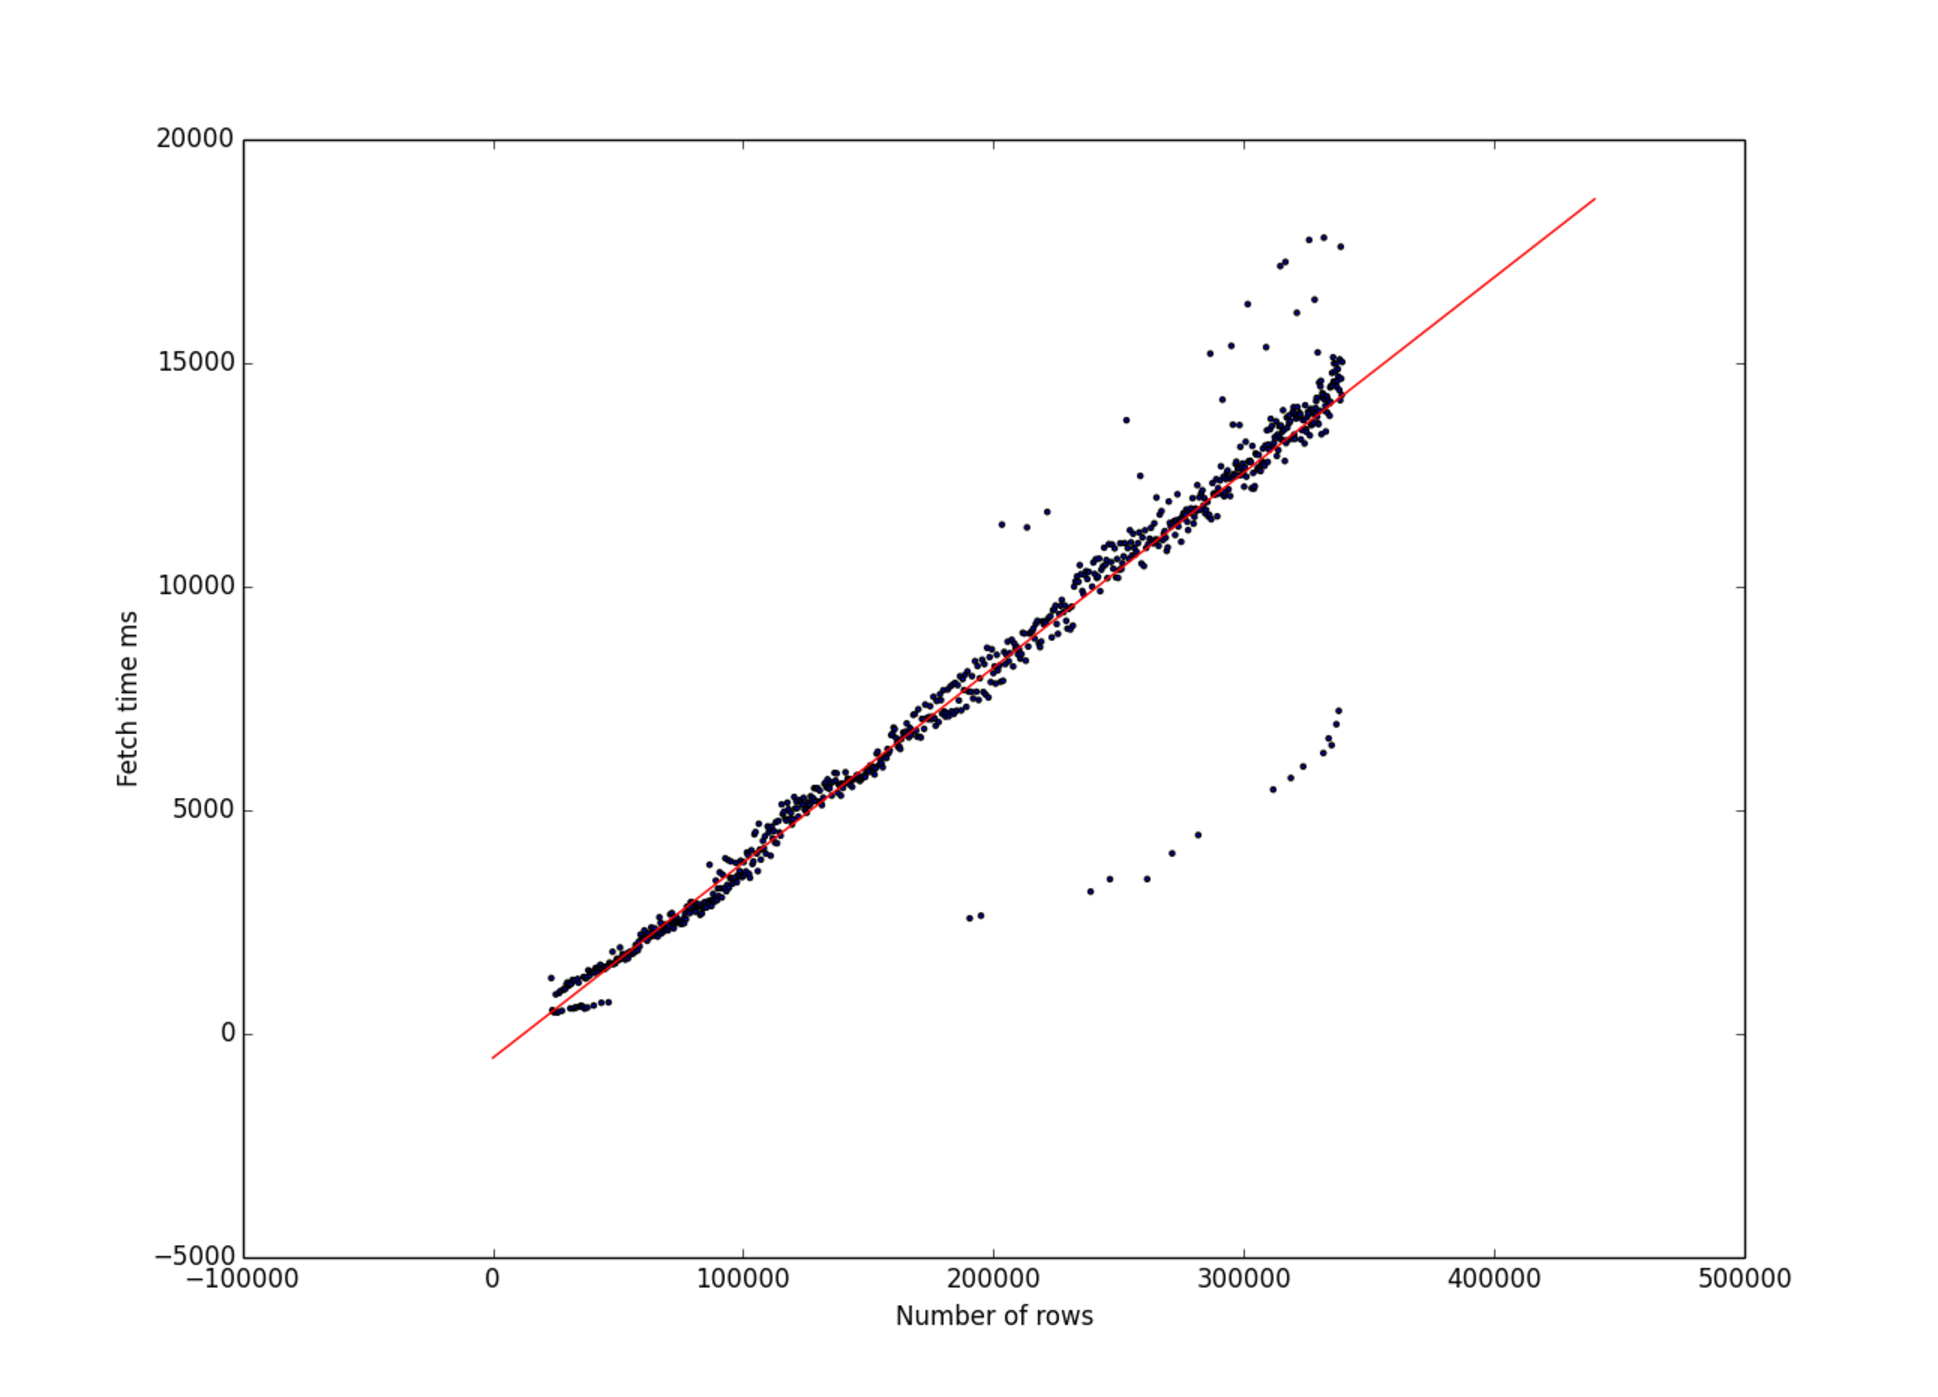
\includegraphics[width=0.5\textwidth] {figures/scale/fetch_time_scale.pdf}
\tightcaption{Time to fetch versus table size.}
\label{fig:fetching-scale}
\end{figure}

\myparatight{Decision making} Once a decision maker has a table, decision making is a matter of multiple lookups for evaluation of each decision. Given that there are $N$ ACs for decision evaluation, and $M$ possible decisions, there are $M \times N$ lookups in a hashmap for a decision to be made. In general, the number of possible decisions is quite small, as are the number of ACs. Consequently, decision making is extremely fast, with an average response time of $.62 \quad ^{+}_{-}\quad .016$ms. See figure~\ref{fig:query-scale}    

\begin{figure}[h!]
\centering
 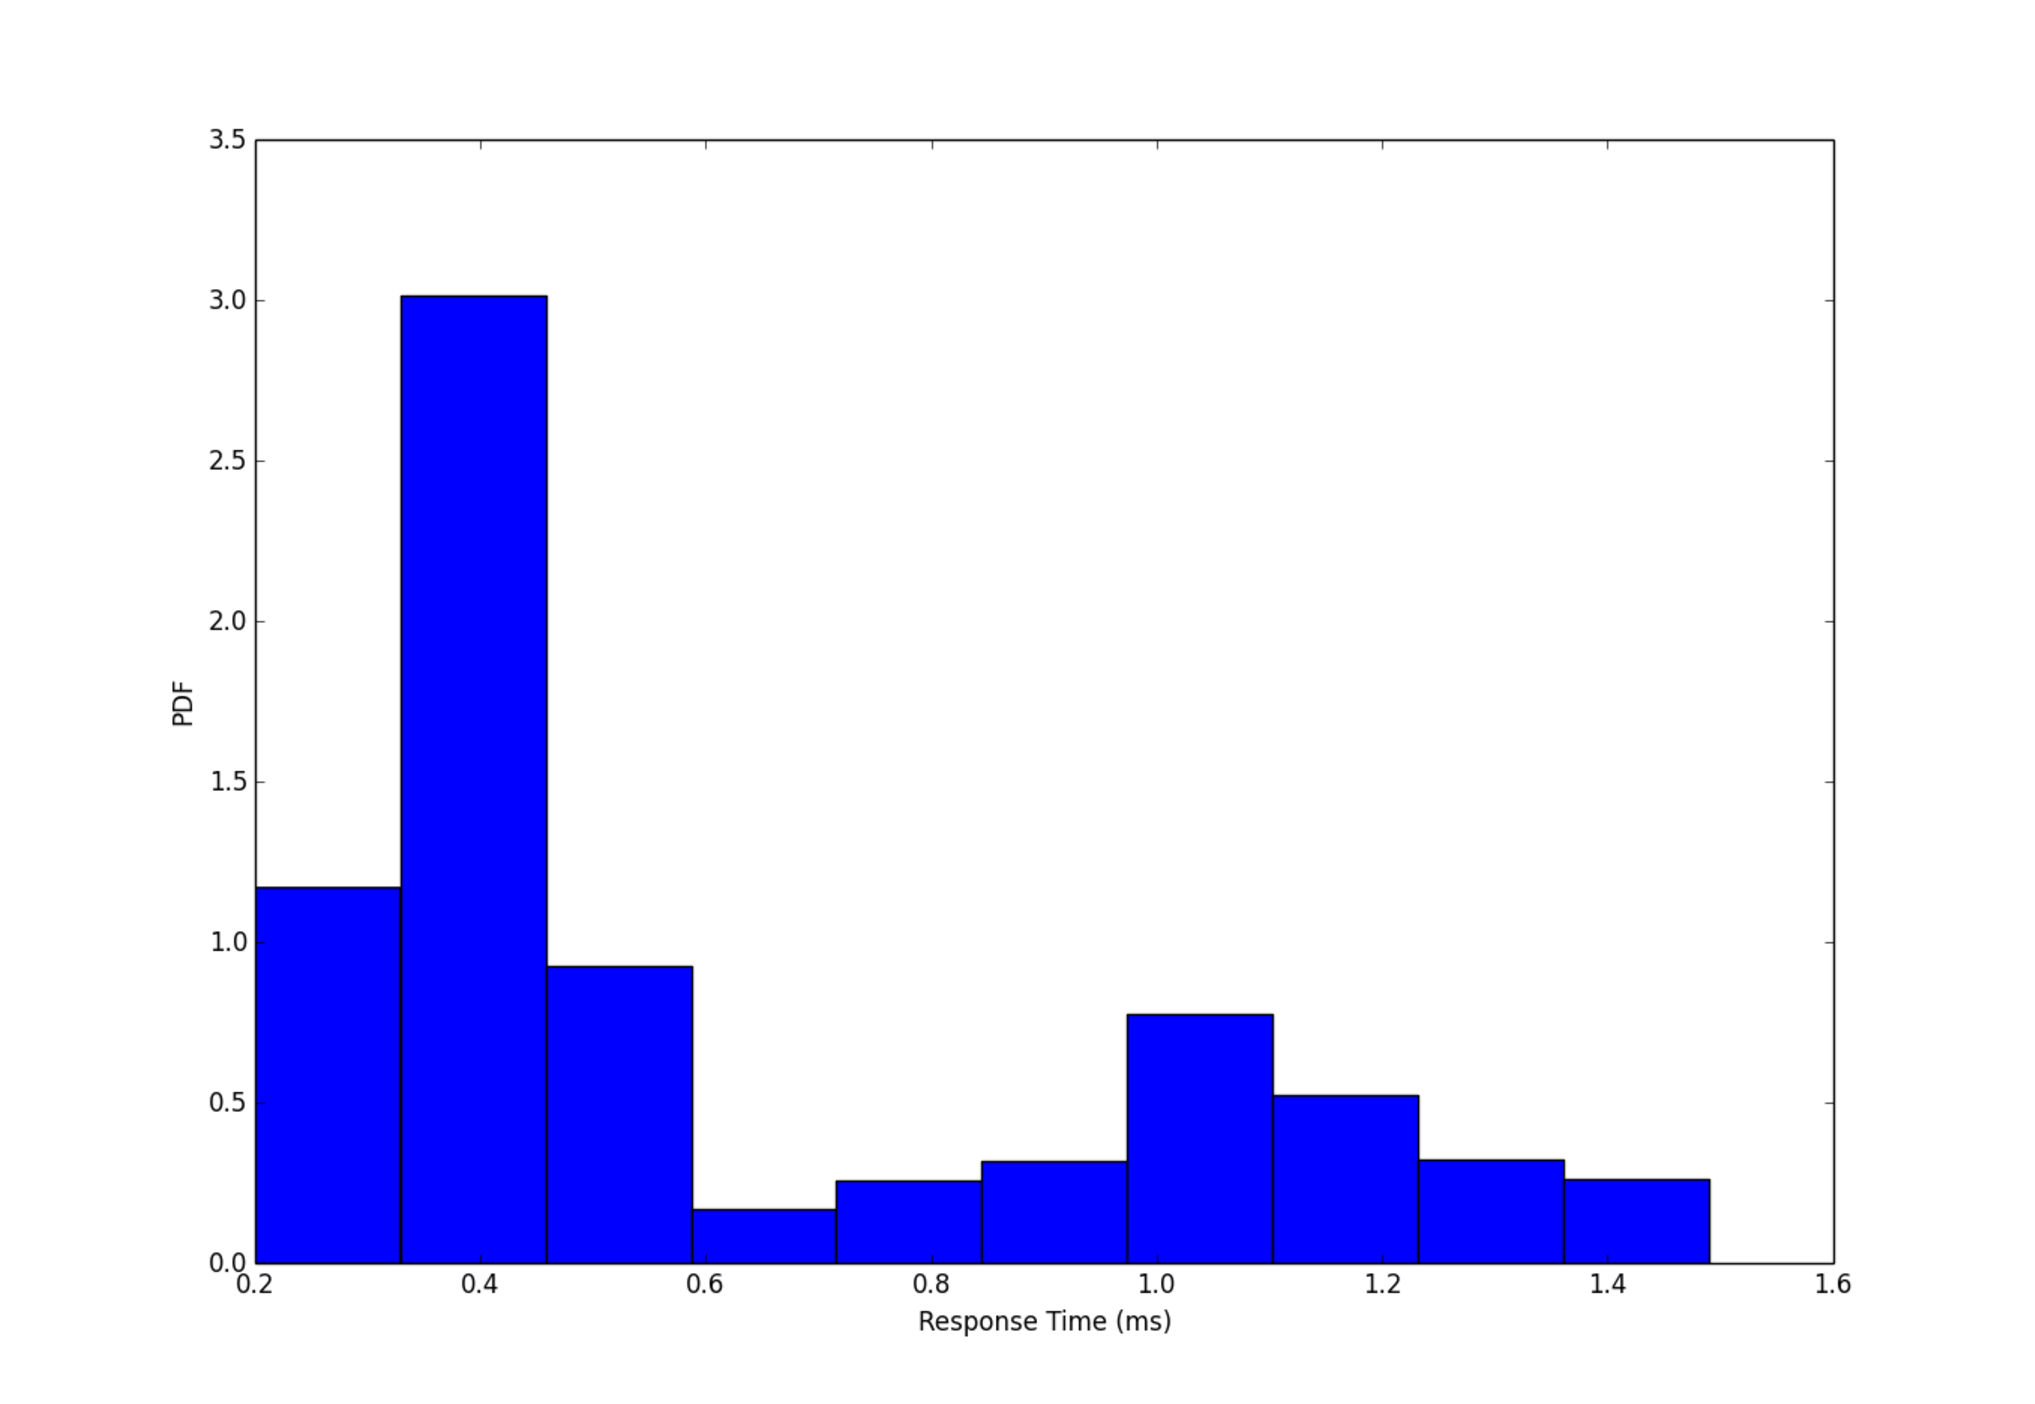
\includegraphics[width=0.5\textwidth] {figures/scale/query_scale.pdf}
\tightcaption{Query times PDF.}
\label{fig:query-scale}
\end{figure}


 
% \tightsection{Scalability}
% The goal of this section is to show that our implementation of the GO backend is scalable for centralized processing, including to continuously collect and process massive client-side measurement and based on the result, make decision for each video session of a large number of viewers. That said, we need to examine 
% \begin{packeditemize}
% \item The general scalability of handling updates and queries of the GO backend, and
% \item The scalability of GO decision making which gets quality samples from quality sample storage and answers query for best decision to querying sessions.
% \end{packeditemize}
% %Note that our implementation leverages several existing techniques (e.g., quality sample aggregation uses Spark). We will also discuss the impact of our particular implementation on the performance.
% 
% \tightsubsection{Backend throughput}
% 
% We need to show that performance (using certain metric) as a function of the number of quality samples (i.e., heartbeats), and the number of session under prediction (i.e., GO precision queries) (and other factors that might impact the scalability of backend throughput). This is to confirm that the backend (excluding GO) is not the bottleneck.
% 
% \tightsubsection{GO scalability}
% 
% The GO implementation has two separate jobs that run in parallel: (1) creating group table -- to fetch the quality samples from quality sample storage, process them into a group table and broadcast the group table to query responders, and (2) decision making -- to answer the query by responders. 
% 
% The delay of creating group table determines the freshness of information based on which the decisions are made. If this step takes $t$ seconds, the decision has to be made based only information that was at least $t$ seconds ago. Delay of decision making is a critical part of the responsiveness of GO backend and potentially a bottleneck of how quickly the client video gets the decision which is very sensitive to video quality when making initial decisions. 
% We should show the performance of both metrics and memory requirement as a function of workload and computational resource as well. 
% \fillme
% 
% 
% 
% 
% \myparatight{Decision making} We then examine the delay of decision making. \fillme

%There are four parts in GO backend that can potentially become performance bottleneck -- user-facing gateway, quality sample storage, quality sample aggregation using ACS, and making individual decisions. To show the scalability, we use micro-benchmark to test their performance as a function of workload (e.g., number of quality samples and queries).


%\tightsection{Quality sample storage}
%Show that quality samples can be processed and stored in an HDFS in parallel. Show runtime as a function number of quality sample updates. \fillme

%\tightsection{Quality sample aggregation}
%Show that quality sample aggregation can be finished in one minute, so that it can be carried every minute. Show both of its running time and memory requirement as a function of number of quality samples and choices of ACS. \fillme

%\tightsection{Making individual decisions}
%Show that once quality samples are aggregated, GO backend can make decsion based on this aggregated information in parallel. Show running time and memory requirement as a function of number of sessions under prediction. \fillme

%\tightsection{User-facing gateway}
%Show that all quality sample updates and queries for best decision will be received and processed immediately. \fillme


\tightsection{Real World Evaluation}
\label{sec:eval}

In this section, we present the implementation and deployment of the GO system (\Section~\ref{sec:impl} and ~\ref{subsec:eval_setup}), and evaluate its performance in real-world (\Section~\ref{subsec:real-world-improvement} and ~\ref{subsec:adaptive-bitrate}). 

The overall improvement is not impressive partly because the deployment is greatly constrained. The deployment only uses one content provider on one platform. 
The content provider enables CDN-level selection across three CDNs where two of them exhibit limited difference in their overall performance during the cause of our experiment,
except in several days we observe performance issues.
%Moreover, the optimization must follow a traffic policy which dictates the total amount of traffic to each CDN. \jc{add a sentence here to explain how GO makes predictive selection under the policy constraints}
However, even with these constraints, we still see arguable improvement. 

\begin{packedenumerate}
    \item We see an overall 7\% reduction in buffering ratio, 4\% increase in average bitrate, and 16\% reduction in number of bitrate switches compared with a random baseline selection algorithm.
    \item We see buffering raito reduction of more than 20\% in several days when a major CDN is experiencing performance degradation.
    \item We show that the initial bitrate chosen by GO is 19\% closer to the dominant bitrate.
\end{packedenumerate}




\begin{figure*}[t!]
\centering
\subfigure[Daily improvement (both metrics)]
{
  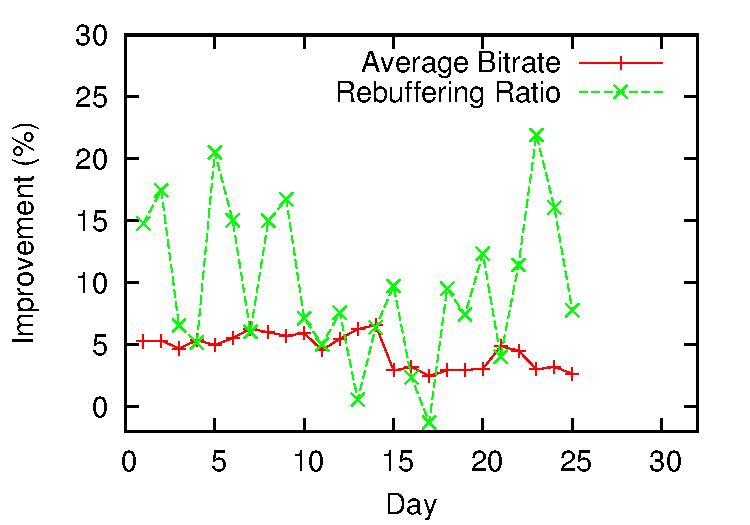
\includegraphics[width=0.3\textwidth] {figures/eval-perfimp.pdf}
  \label{subfig:buffering-and-bitrate}
}
\subfigure[Buffering ratio (\%): GO vs. per-CDN]
{
	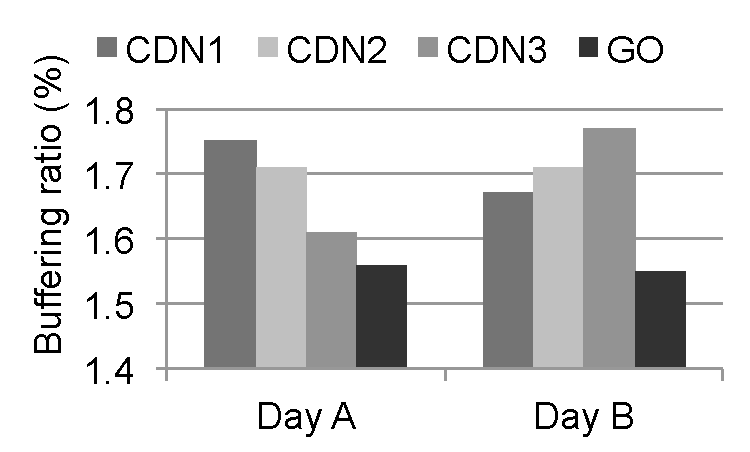
\includegraphics[width=0.3\textwidth]{figures/ab-testing-figures/bufferingratio-new.pdf}
	\label{subfig:eval-case-study:bufferingratio}
}
\subfigure[Avg. bitrate (Kbps): GO vs. per-CDN]
{
	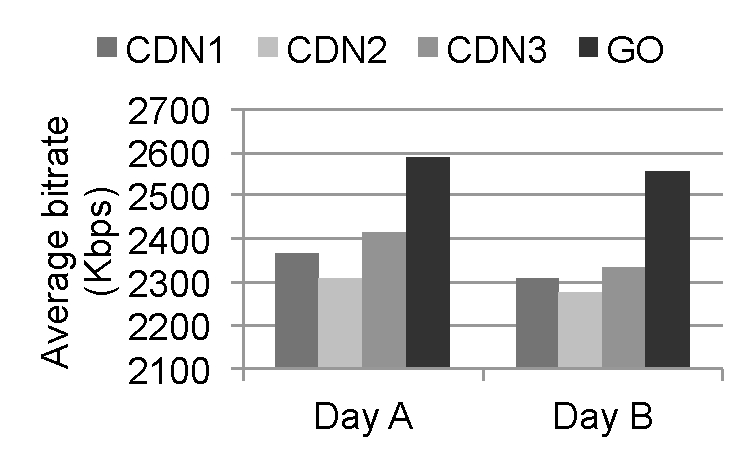
\includegraphics[width=0.3\textwidth]{figures/ab-testing-figures/averagebitrate-new.pdf}
	\label{subfig:eval-case-study:averagebitrate}
}
\tightcaption{Performance Metrics and Improvement from GO}
\label{fig:perf-impr}
\end{figure*}



\tightsubsection{System Implementation \& Scalability}
\label{sec:impl}
We first present the high level GO implementation. While there are much details in building GO system, we focus on the two main components: data processing and decision making. Paramount in our implementation was the need to make very rapid decisions, as any extra delay in decision making could impact performance of the client making the request. This meant that the vast majority of prediction information needed to be precomputed. This resulted in an implementation that involves two parts: computation and updating of a group table every minute, and broadcasting of the table out to servers close to the clients.

\myparatight{Creating group table} Group table generation is essentially the process of aggregating quality samples into partitions of different ACs, and then computing summary statistics for each partition (e.g., mean and standard error of mean).
Our implementation uses Spark~\cite{spark} as the underlying compute framework, and the problem can be captured in a single map-reduce stage. 
Quality samples are loaded in parallel from an HDFS source~\cite{hadoop} and distributed amongst the cluster in form of Resilient Distributed Datasets (RDD)~\cite{zaharia2012resilient}. 
%Each node then maps its share of quality samples to a set of preliminary buckets. Common buckets are then shuffled across the cluster and the results are aggregated and collected onto a master machine. 
Currently it takes GO system 12 seconds to process 500K partitions on a 4-node cluster with a total of 64 cores and 512G memory, without riguous performance optimization.
It is also worth noting that all steps involved in creating the table are horizontally scalable.


\myparatight{Broadcasting group table} The resulting table is broadcasted wholesale out to a large number of decision makers (DMs) closer to video clients in multiple POPs by way of a distributed messaging system~\cite{kreps2011kafka}. The bottleneck here is bandwidth, because at minimum, we need to ship one table copy to each POP where we deployed decision makers. We believe this is justified by providing quick response to video players. Our current GO table size is 50MB for 500K entries, with an update frequency of one minute, the bandwidth required is 0.83Mbps per POP. We would like to note that we have not optimized serialization and deserialization in terms of size.

\myparatight{Decision making} Once a decision maker has a table, decision making is a matter of running the prediction algorithm for evaluation of each decision. Given that there are $N$ ACs for decision evaluation, and $M$ possible decisions, there are $M \times N$ lookups for a decision to be made. The decision making process is horizontally scalable by adding more decision makers, and in general, decision making is extremely fast. The average response time from current GO system is $0.62 ^{+}_{-} 0.016$ms with 3 decision makers (both query per second and CPU utilization are low on the decision makers), which is insignificant compared to RTT in Internet.

In summary, we implemented GO which is both scalable and provide good system-level performance.


\tightsubsection{Deployment Setup}
\label{subsec:eval_setup}

GO is deployed on one content provider with short-form videos (5 minutes) on iOS device (both iPhone and iPad). 
HLS protocol is running on the iOS device and our GO system decides the initial CDN and bitrate, while Apple player employs adaptive 
bitrate switching algorithm to change the bitrate during the video session (without CDN switch). 

The results are collected from Jan 1st, 2014 to Jan 25th, 2014 (total of 25 days) with 26.1 million sessions (870K sessions on average per day).
There are three CDNs in this experiement, and 5 bitrate levels (from 700Kbps to 3.5Mbps). We evaluate two algorithms: {\it randomized} baseline and {\it optimized} (by GO).


\tightsubsection{Quality Improvement}
\label{subsec:real-world-improvement}

Figure~\ref{subfig:buffering-and-bitrate} shows the performance improvement of GO over randomized baseline on two quality metrics of
buffering rate and average bitrate over the 25-day period. The overall improvement over the entire 25-day period is 7\% reduction in buffering ratio and 4\% increase in 
average bitrate. The figure also shows that performance improvement varies by day, depending on how different the performance of each CDN. 
In fact, we noticed that, for this site, performance of multiple CDNs tend to become close to each other
during weekends where CDNs are likely under-loaded and thus, we see no noticeable improvement from GO in those days. 
On the other hand, on day 25, we noticed a big performance improvement of more than 20\%. After investigation,
we found that a major CDN was experiencing performance issues that lasts for more than one day. 

To further illustrate GO's ability to handle spatial and temporal variation, 
we look into some particular examples and compare GO with each CDN. Figure~\ref{subfig:eval-case-study:bufferingratio} and~\ref{subfig:eval-case-study:averagebitrate} show two example days in which three CDNs performed differently.  For example, in terms of buffering ratio, CDN3 was the best on Day A and CDN1 was the best on Day B. 
We can see that in both Day A and B, GO managed to outperform the best-performing CDN in both average bitrate 
and buffering ratio. This suggests that GO was not only looking for the globally best CDN, but also 
differentiated CDN performance in finer granular partition.

%\xil{add a spatial diversity graph}



\tightsubsection{Adaptive Bitrate Behavior}
\label{subsec:adaptive-bitrate}

Previous research (e.g., ~\cite{user-adaptive,videoqoe}) shows that bitrate switching rate has an impact on video experience. In this section, we evaluate the adaptive 
bitrate switching behavior with and without GO. 

\myparatight{When Do Adaptive Bitrate Switches Happen?}
We first take a look at when do adaptive bitrate switches happen. Figure~\ref{fig:switch-time-dist} shows that the 
majority of switches happen at the beginning of the video plays, i.e., around 60\% of the switches 
happen within 20\% of the video duration. Switching behavior varies for different adaptive bitrate algorithms, and we do not 
claim such observation apply to all algorithms.

To account for viewers leaving in the middle of the video play, note that the x-axis is chosen as the percentage of actual 
video play duration instead of content length. 
In this figure, we include another content provider who provides long-formed content (one hour) on iOS platforms, and we have similar observations. This suggests the importance of initial bitrate selection, through which viewers can have a smoother video playback experience.

\begin{figure}[h!]
\centering
 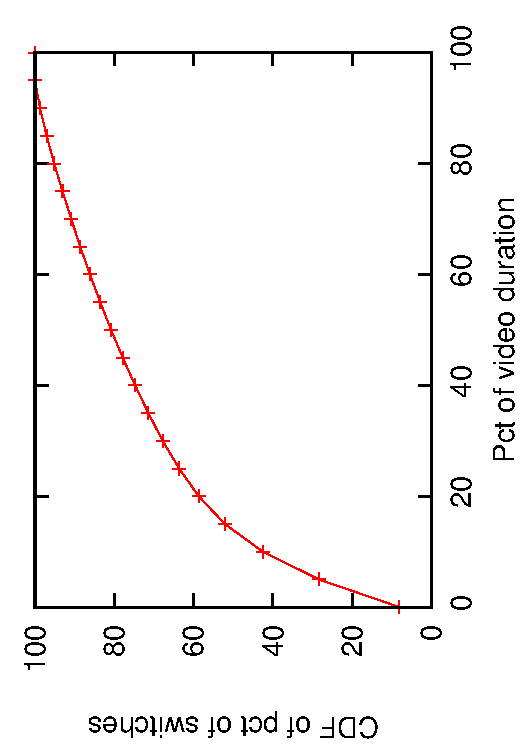
\includegraphics[width=0.3\textwidth] {figures/switch-time-dist.pdf}
\tightcaption{When do adaptive bitrate switches happen? \jc{what's the threshold between long and short form content}}
\label{fig:switch-time-dist}
\end{figure}



\myparatight{Reducing Number of Bitrate Switch}
Next let us evaluate the switching stability by looking at the number of switches within the first minute of the video play.
We chose one minute because the videos are 5 minutes long and first minute account for 60\% of the switches (see Figure~\ref{fig:switch-time-dist}). 
Since HLS has 10 second video chunks, the maximum number of switches is 6 in this case.
Figure~\ref{subfig:reduce-switch} shows the number of bitrate switches for optimized and random decisions. 
Overall GO can reduce the number of switches by 16\%, and it also increases the number of non-switching-interrupted sessions 
(sessions that experience no switching) by 10\%.
It is possible the reason GO reduces the number of switches is shorter video plays, however, we observed engagement lift
(viewers watch longer because of better quality) at the same time of reduction in number of switches.



\begin{figure}[h!]
\centering
\subfigure[Number of bitrate switches \jc{Xi, revert to last version?}]
{
  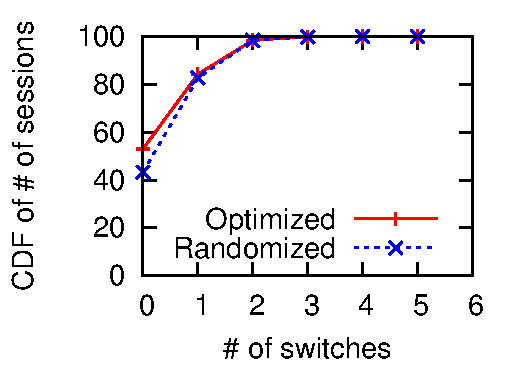
\includegraphics[width=0.24\textwidth] {figures/eval-reduceswitch.pdf}
  \label{subfig:reduce-switch}
}
\hspace{-0.6cm}
\subfigure[Initial vs. dominant bitrate]
{
  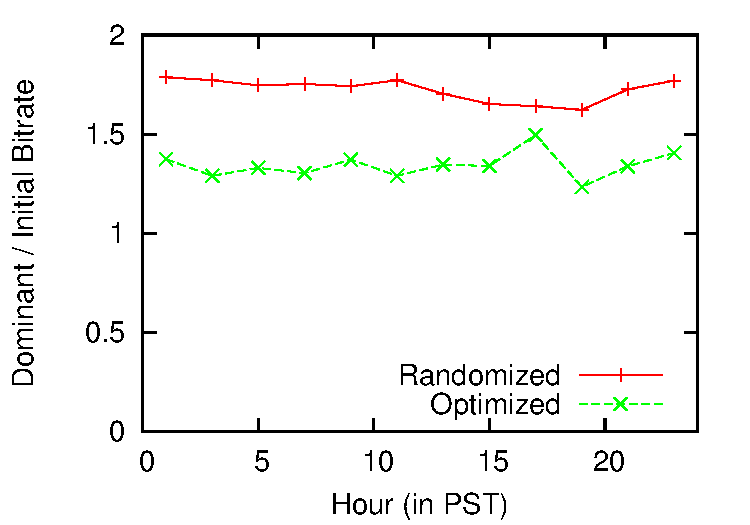
\includegraphics[width=0.24\textwidth] {figures/eval-initvsdom.pdf}
  \label{subfig:initvsdom}
}
\tightcaption{GO improves bitrate adaptation by selecting a better initial bitrate and thus reducing number of bitrate switches.}
\label{fig:bitrate-stability}
\end{figure}


\myparatight{Dominant vs. Initial Bitrate}
Another metric we use to evaluate GO initial bitrate selection is the rate between dominant bitrate and initial bitrate. Dominant bitrate
is the bitrate that the sessions plays for the longest duration, and ideally this number should be 1. Figure~\ref{subfig:initvsdom} shows the ratio of initial bitrate to dominant bitrate. Overall GO is 19\% closer to the dominant bitrate than randomized bitrate selection. 
The figure also shows that for 60\% of the GO-optimized sessions, the initial bitrate selected by GO is almost the same as the dominant bitrate.
%We would like to emphasize again that GO does not make the improvement at the price of engagement, and GO in fact improves engagement.

In summary, our early experience of GO in the real world suggests that it is a promising step towards the global control plane.


\tightsection{Related Work}
We briefly highlight two areas of research to place our work in context.

\tightsubsection{QoS of Internet video}
\myparatight{Quality metrics} 
A key aspect in  video delivery is to optimize user-perceived  quality of experience.  There is evidence that
users are sensitive to buffering ratio (e.g., \cite{sigcomm11}) and frequent changes in bitrate (e.g.,~\cite{user-adaptive,videoqoe}). More recent studies show a more causal relationsihpe betwen quality and user engagement~\cite{akamai-imc12}. The design of a good QoE metric (e.g., \cite{qscore}) is still an active area of research. As our understanding of video QoE matures, we can extend GO to be QoE-aware (as suggested in ~\cite{sekar2012quest})

\myparatight{Client-side adaptation} This includes the work on identifying problems existing in client-adaptation algorithms (e.g.,~\cite{mmsys2011cisco}), interation between player logic and TCP (e.g.,~\cite{usenix12_ghobadi,nossdav12_esteban}), and better bitrate adaptation algorithm to improve quality (e.g.,~\cite{nossdav12_akhshabi,festive}). GO can be considered as an enhancement to client-side adaptation by making decisions based on the information collected from massive clients.

\myparatight{CDN and server selection} These efforts have demonstrated inefficiencies in CDN and server selection strategies~\cite{youtubecdn,youtube-infra}, and studied various techniques to improve video quality, including cross-CDN optimization (e.g., ~\cite{sigcomm12,sigcomm12cdnmulti}), CDN federation (e.g.,~\cite{peterson2013framework}) and the use of ISP-CDN (e.g., ~\cite{yu2012tradeoffs,frank2013pushing}).  While GO currently focuses on quality improvement via better CDN and bitrate selection, we expect GO and its techniques to help these techniques make more accurate decisions.

\myparatight{Other video measurement}  There is a large  literature in measuring the performance of video delivery quality including content popularity and access patterns (e.g.,~\cite{youtube-imc07}\cite{plissonneau2012longitudinal}) and flash crowds during highly popular events (e.g.,~\cite{beijing-imc09}). Using a dataset that provides similar panoramic view, ~\cite{jiang2013shedding} studies the structure of video quality problems in more dimensions (e.g., content provider and video type). GO's attribute-based prediction algorithm extends a similar structural analysis to quality prediction and study the effectiveness of predicting not only whether a session has quality problems, but also its quality.

\tightsubsection{Global optimization}

\myparatight{Control plane and centralized decisions} There is a long line of work in which the control plane is separated from the data plane (e.g.,~\cite{rcp,onix,4d,openflow}) and they focus on physical networks and the objectives are often packet forwarding behaviors and policy compliance in routing. In contrast, GO optimize application-level applications by controlling client-side devices and the objectives are performance or quality metrics.  

\myparatight{Controller scalability and fault-tolerance} By making control decisions at a centralized point, SDN and similar centralized systems create a single point-of-failure at the controller and previous research has proposed many related techniques to build a scalable and fault-tolerant controller/backend (e.g., ~\cite{tootoonchian2012controller,yan2007tesseract}). The implementation of GO backend leverages many existing techniques to make it scalable, efficient and resillient, including Spark~\cite{spark}, Hadoop and ...

\myparatight{Information sharing} Information sharing has been used to make more informed decision in networking research since a decade before. These works (e.g.,~\cite{stemm2000network} and more recently, \cite{choffnes2010crowdsourcing}) explore the feasibility of a wide area measurement infrastructure to monitor network-level performance and inform application-level decisions. Sharing across multiple applications within a host is also studied (e.g., \cite{balakrishnan1999integrated}). While these works try to optimize quality like GO, they require dedicated centralized sharing or distribute sharing infrastructure, and we rely only on instrumentation within video players to measure a wide-area performance by leveraging the dominance of video traffic in today's Internet. Moreover, GO deals with more attributes and requires a more complex model than these works whose network models do not include application-specific attributes, e.g., content provider or streaming protocols.

\tightsection{Discussion}

While our results look promising, the magnitude of the improvements
may seem underwhelming. However, we believe that this is not due to
the lack of potential of our approach, but it merely comes down to the
inherent limitations that are typical to any first instantiation of a
radical approach. In the reminder of this section, we consider some of
these limitations which, when removed, will result in much higher
improvements.

\myparatight{Midstream selection} Today, GO makes decisions only at
the sessions' start times. For a long session this can be far from
optimal, as, for example, the quality of the selected CDN may degrade
during the session's lifetime. We are currently working on making the
decisions during the midstream, as well. Note that in this case, the
prediction is equally important, as switching to a new CDN is not
guaranteed to increase the quality, especially if the quality
degradation is due to the last mile or due to the client inability to
render at a high bitrate.

\myparatight{Leveraging network and CDN information} GO makes
decisions based on client side information only. While clients provide
the most accurate information regarding the quality experienced by
users, this information is not always optimal when making
decisions. The decision process can be considerably improved if GO
were to leverage information from other entities in the distribution
ecosystem, including CDN servers, caches, and routers. Using such
information, GO could significantly improve the prediction
accuracy. For example, GO could learn much faster that a CDN server is
overloaded by getting load information directly from that server than
infering this information from clients that experience quality issues
when connected to that server.

\myparatight{Finer grain selection} Currently, GO selects the resource
 at the CDN granularity. This means that GO can't do much if the CDN
 redirects the client based on its location (e.g., IP address) and the
 servers the CDN redirects the client to are congested. However, if
 the client were able to specify the servers to stream from, GO could
 avoid the overloaded servers and dramatically increase the
 quality. We believe that we will soon have the ability to perform
 such fine grain selection, as CDNs are incentivized to expose such
 fine grain information to clients. Indeed, a CDN operator will prefer
 that a quality impacted client to move to other servers in the same
 CDN rather than migrate to a different CDN! Furthermore, an ISP CDN
 that also runs its own software on setop boxes or other user devices
 would be in the perfect position to run a GO like algorithm that
 makes decisions at server granularity.

\myparatight{Join network optimization} The decisions made by GO are
oblivious to the network conditions. As such, there is little GO can
do if the network is congested. GO can perform considerably better if,
in addition to the endpoints, were able to select the network
paths. Again, this would make perfect sense in the context of an ISP
CDN where the ISP controls both the network and the distribution
infrastructure.


%\myparatight{Behaviore-related attributes}


%\myparatight{Finer granular server selection}

%\myparatight{Traffic load balance}

{\scriptsize
\bibliographystyle{abbrv}
\bibliography{adaptation,sigcomm2011,sigcomm2012,sigcomm2013,conext13}
}

\appendix
\tightsection{Evaluation methodology}
Throughout this paper we make use of a methodology we call ``counterfactual testing'', or CT, for producing unbiased estimates of the impact of CDN selection algorithms on quality outcomes.  CT is a relative of A/B testing, a well-known method for producing estimates of the effects of decisions (see, for example, \cite{kohavi2009online} for a case study of its use at Microsoft).  Like A/B testing it relies crucially on randomization of decisions, but unlike A/B testing it permits retrospective evaluation of decision-making algorithms, at the cost of reduced statistical efficiency (i.e. the need for more data).  \henry{It is quite likely that a similar method is used to test treatment targeting strategies in clinical trials, and we should cite it if it exists, but I cannot find any literature on this.}

The idea is that we can accurately evaluate sessions whose counterfactual decisions happen to match their actual decisions, since we observe their outcomes.  By dropping from our dataset all sessions whose counterfactual decisions do not match their actual decisions, we identify a dataset over which we can feasibly compute average quality under the counterfactual decisions.  Assuming the actual decisions are random, the choice to drop a session in this way is random, which means that the procedure is equivalent to randomly dropping some of the data.  A simple reweighting step, which corrects for the different probability of dropping sessions with different counterfactual decisions, permits recovery of unbiased results.  This procedure works for arbitrary sets of counterfactual decisions, as long as the actual decisions in the dataset were taken randomly.

Let $J \subset \mathbb{N}$ be a set of indices for the possible decisions, which we assume for simplicity is the same for each session.  Let $d_i \in J$ be the decision made for the $i$th session, $0 \leq 0 < N$, and $\hat{d}_i \in J$ be the simulated (counterfactual) decision for the same session.  Let $q_i \in \mathbb{R}$ be the quality outcome actually observed for that session, and let $\hat{q}_i \in \mathbb{R}$ be the (unknown) quality outcome we would have observed if decision $\hat{d}_i$ had been taken for that session.  It is assumed that the $d_i$ were chosen mutually independently and further that $d_i$ is independent of all observable attributes of session $i$.  We also assume that each $d_i$ has known distribution $P_i$ and that $P_i$ assigns strictly positive probability to each possible decision.  All of these assumptions are met if, for example, the decisions are chosen uniformly at random for each session.  The most restrictive assumption is that there are no interactions among the effects of decisions; that is, we assume $q_i$ is independent of $d_j$ for $i \neq j$ and $\hat{q}_i$ is independent of $\hat{d}_j$ for $i \neq j$.  This assumption is certainly violated to some extent, though a similar assumption is made in A/B testing.

Let $\bar{Q}$ be the average quality in the counterfactual situation, $\frac{1}{N} \sum_{i < N} \hat{q}_i$.  Let $\hat{Q}$ be the average quality reported by CT, and let $1[x] = 1$ if $x$ is true and $0$ otherwise.  Then $\hat{Q}$ is computed as follows:
\begin{align*}
  \hat{Q} &= \frac{1}{N} \sum_{i < N} \frac{1}{P_i(\hat{d}_i)} 1[d_i = \hat{d}_i] q_i
\end{align*}
Sessions for which counterfactual decisions do not match actual decisions are dropped, and the remaining sessions are weighted according to their probability of being dropped.  It is straightforward to verify that $\hat{Q}$ is an {\it unbiased} estimate of $\bar{Q}$ for any $N$ (it is essentially an estimate of $\bar{Q}$ using {\it importance sampling}, which is unbiased \cite{something}):
\begin{align*}
    \E[\hat{Q}] &= \E[\frac{1}{N} \sum_{i < N} \frac{1}{P_i(\hat{d}_i)} 1[d_i = \hat{d}_i] q_i] \\
    &= \frac{1}{N} \sum_{i < N} \frac{1}{P_i(\hat{d}_i)} \E[1[d_i = \hat{d}_i] q_i] \\
    &= \frac{1}{N} \sum_{i < N} \frac{1}{P_i(\hat{d}_i)} \E[1[d_i = \hat{d}_i] \hat{q}_i] \\
    &= \frac{1}{N} \sum_{i < N} \frac{1}{P_i(\hat{d}_i)} P_i(\hat{d}_i) \hat{q}_i \\
    &= \frac{1}{N} \sum_{i < N} \hat{q}_i \\
    &= \bar{Q}
\end{align*}

Unbiasedness means that CT does not on average (i.e. over many hypothetical repetitions of randomized decision-making) over- or underestimate $\bar{Q}$.  However, like A/B testing, it is still subject to estimation error, which depends on the sample size.  By dropping many sessions to compute $\hat{Q}$, CT reduces the effective sample size, exacerbating estimation error.  Confidence intervals reported in this paper incorporate this additional uncertainty.

\end{document}
